%%%%%%%%%%%%%%%%%%%%%%%%%%%%%%%%%%%%%%%%%
% Masters/Doctoral Thesis 
% LaTeX Template
% Version 2.5 (27/8/17)
%
% This template was downloaded from:
% http://www.LaTeXTemplates.com
%
% Version 2.x major modifications by:
% Vel (vel@latextemplates.com)
%
% This template is based on a template by:
% Steve Gunn (http://users.ecs.soton.ac.uk/srg/softwaretools/document/templates/)
% Sunil Patel (http://www.sunilpatel.co.uk/thesis-template/)
%
% Template license:
% CC BY-NC-SA 3.0 (http://creativecommons.org/licenses/by-nc-sa/3.0/)
%
%%%%%%%%%%%%%%%%%%%%%%%%%%%%%%%%%%%%%%%%%

%----------------------------------------------------------------------------------------
%	PACKAGES AND OTHER DOCUMENT CONFIGURATIONS
%----------------------------------------------------------------------------------------

\documentclass[
% The default document font size, options: 10pt, 11pt, 12pt
11pt, 
% Two side (alternating margins) for binding by default, uncomment to switch to one side
oneside,
% ngerman for German
english,
% Single line spacing, alternatives: singlespacing, onehalfspacing or doublespacing
onehalfspacing,
% Uncomment to enable draft mode (no pictures, no links, overfull hboxes indicated)
%draft,
% If the document is nolistspacing, onehalfspacing or doublespacing, uncomment this to set spacing in lists to single
onehalfspacing,
% Uncomment to add the list of figures/tables/etc to the table of contents
%liststotoc,
% Uncomment to add the main table of contents to the table of contents
%toctotoc,
% Uncomment to add space between paragraphs
parskip,
% Uncomment to not load the hyperref package
%nohyperref,
% Uncomment to get a line under the header
headsepline,
% Uncomment to place the chapter title next to the number on one line
chapterinoneline,
% Uncomment to change the layout of the declaration, abstract and acknowledgements pages to match the default layout
%consistentlayout,
% The class file specifying the document structure
]{MastersDoctoralThesis}

% Required for inputting international characters
\usepackage[utf8]{inputenc}

% Output font encoding for international characters
\usepackage[T1]{fontenc}
\usepackage{textcomp} % support the degree symbol

% Use the Palatino font by default
\usepackage{mathpazo}

% Use tu justify paragraphs
\usepackage{ragged2e}

% Use the bibtex backend with the authoryear citation style (which resembles APA)
\usepackage[backend=biber,natbib=true]{biblatex}
% MLA, APA, or IEEE? - https://www.overleaf.com/learn/latex/Biblatex_citation_styles
%\usepackage[style=apa, backend=biber]{biblatex}

% The filename of the bibliography
\addbibresource{references.bib}

% Required to generate language-dependent quotes in the bibliography
\usepackage[autostyle=true]{csquotes}

% to set default colours
\usepackage{xcolor}
\definecolor{mygray}{gray}{0.5}

% for gantt charts
\usepackage{tikz}
\usepackage{gantt}

% to rotate pages in landscape
\usepackage{lscape}

% equation arrows with text
\usepackage{amsmath}

% insert degree celsius symbol
\usepackage{textcomp}

%----------------------------------------------------------------------------------------
%	MARGIN SETTINGS
%----------------------------------------------------------------------------------------

\geometry{
	paper=a4paper,      % Change to letterpaper for US letter
	inner=2.5cm,        % Inner margin
	outer=3.8cm,        % Outer margin
	bindingoffset=.5cm, % Binding offset
	top=1.5cm,          % Top margin
	bottom=1.5cm,       % Bottom margin
	%showframe,         % Uncomment to show how the type block is set on the page
}

%----------------------------------------------------------------------------------------
%	THESIS INFORMATION
%----------------------------------------------------------------------------------------

% Your thesis title, this is used in the title and abstract, print it elsewhere with \ttitle
\thesistitle{The Impact of Urban Agriculture in Sustainable Cities.}

% Your supervisor's name, this is used in the title page, print it elsewhere with \supname and \cosupname
\supervisor{Diego Fabián \textsc{Lozano} García}
\cosupervisor{Rosa María \textsc{López} Franco}

% Your examiner's name, this is not currently used anywhere in the template, print it elsewhere with \examname
\examiner{}

% Your degree name, this is used in the title page and abstract, print it elsewhere with \degreename
\degree{Leadership for Sustainable Development}

% Your name, this is used in the title page and abstract, print it elsewhere with \authorname
\author{
\textbf{A01169284} - Bruno González Soria \\
\textbf{A01212611} - Antonio Osamu Katagiri Tanaka \\
\textbf{A01750267} - Carlos Cardoso Isidoro
}

% Your address, this is not currently used anywhere in the template, print it elsewhere with \addressname
\addresses{Estado de México, Atizapan de Zaragoza}

% Your subject area, this is not currently used anywhere in the template, print it elsewhere with \subjectname
\subject{Nanotechnology}

% Keywords for your thesis, this is not currently used anywhere in the template, print it elsewhere with \keywordnames
\keywords{sustainable cities, compact cities, urban agriculture, urban land use planning}

% Your university's name and URL, this is used in the title page and abstract, print it elsewhere with \univname
\university{\href{https://tec.mx/}{Instituto Tecnonólogico y de Estudios Superiores de Monterrey}}

% Your university's campus name and URL, this is used in the title page and abstract, print it elsewhere with \campusname
\campus{\href{https://tec.mx/}{Campus Estado de México}}

% Your department's name and URL, this is used in the title page and abstract, print it elsewhere with \deptname
\department{\href{https://tec.mx/}{School of Engineering and Sciences}}

% Your research group's name and URL, this is used in the title page, print it elsewhere with \groupname
\group{\href{https://www.medinadora.com/people}{ITESM \campusname}}

% Your faculty's name and URL, this is used in the title page and abstract, print it elsewhere with \facname
\faculty{\href{https://samp.itesm.mx/Programas/VistaPrograma?clave=MNT16&modoVista=Default&idioma=ES&cols=0}{Faculty: Nanotechnology}}

\AtBeginDocument{
\hypersetup{pdftitle=\ttitle}          % Set the PDF's title to your title
\hypersetup{pdfauthor=\authorname}     % Set the PDF's author to your name
\hypersetup{pdfkeywords=\keywordnames} % Set the PDF's keywords to your keywords
}

\begin{document}

% Use roman page numbering style (i, ii, iii, iv...) for the pre-content pages
\frontmatter

% Default to the plain heading style until the thesis style is called for the body content
\pagestyle{plain} 

%----------------------------------------------------------------------------------------
%	TITLE/COVER PAGE
%----------------------------------------------------------------------------------------

\begin{titlepage}
\begin{center}

\vspace*{.06\textheight}
{\scshape\LARGE \univname\par} % University name

%\begin{center}

\includegraphics[width=0.15\textwidth]{./Figures/uniLogo.png}
%\end{center}

\vspace{0.5cm}
\textsc{\Large Final Project Report}\\[0.5cm]      % Thesis type

\HRule \\%[0.5cm]                           % Horizontal line
{\huge \bfseries \ttitle\par}\vspace{0.0cm} % Thesis title
\HRule \\[0.5cm]                            % Horizontal line
 
\begin{minipage}[t]{0.4\textwidth}
\begin{flushleft} \large
\emph{Author(s):}\\

% Author name - remove the \href bracket to remove the link
%\href{https://linkedin.com/in/osamu-katagiri-84b2b940/}{\authorname} \\
\authorname
\end{flushleft}
\end{minipage}
\begin{minipage}[t]{0.4\textwidth}
\begin{flushright} \large
\emph{Instructor(s):} \\
% Supervisor name - remove the \href bracket to remove the link
%\href{http://www.doramedina.com}{\supname}
\supname

% Supervisor name - remove the \href bracket to remove the link
%\href{https://www.medinadora.com/}{\cosupname}
\cosupname
\end{flushright}
\end{minipage}\\[0.5cm]

\vfill

\large \textit{A project report submitted in fulfillment of the requirements\\ for the course of
% University requirement text
\degreename}\\[0.25cm]
\textit{in}\\[0.25cm]
% Research group name and department name
\groupname\\\deptname\\[1cm]
 
\vfill

% Address and Date
{\addressname \text{, } \large \today}\\[4cm]
% University/department logo - uncomment to place it
%
\includegraphics{./Figures/uniLogo.png}
 
\vfill
\end{center}
\end{titlepage}

%----------------------------------------------------------------------------------------
%	ABSTRACT PAGE
%----------------------------------------------------------------------------------------

\begin{abstract}
\addchaptertocentry{\abstractname} % Add the abstract to the table of contents

The debate on the role of urban agriculture in the sustainable city discourse remains unresolved in the conventional literature. Therefore, the purpose of this study was to review relevant literature to clarify the role of urban agriculture in sustainable cities. The search for literature was guided by themes such as: a) urban agricultural practices, b) indicators for the measurement of sustainable cities, c) economic, social and environmental benefits of urban agriculture, and d) negative effects of urban agriculture on the city. The results from a synthesis of the literature indicate that urban agriculture supports the economic, social and environmental sustainability of cities. However, if the discussion gives credence to only the economic dimension of sustainability, then urban agriculture loses the debate. This is because the economic benefits of prime city land that is used used for nonagricultural purposes (such as commercial or industrial) is profound. However, the social and environmental functions of responsible urban agriculture, particularly in reducing the rift between urbanisation and nature, may be difficult to quantify. These social and environmental functions underscore the importance of urban agriculture in the city landscape. The paper concludes by arguing that focussing on only economic sustainability in the urban agriculture-sustainable city discourse is a travesty of the idea of sustainable development. The paper presents practical steps that can be taken to preserve agriculture in cities towards their sustainability. \\

\noindent
\textbf{keywords:} \keywordnames
\end{abstract}

%----------------------------------------------------------------------------------------
%	LIST OF CONTENTS/FIGURES/TABLES PAGES
%----------------------------------------------------------------------------------------

\tableofcontents % Prints the main table of contents

\listoffigures % Prints the list of figures

%\listoftables % Prints the list of tables

%----------------------------------------------------------------------------------------
%	ABBREVIATIONS
%----------------------------------------------------------------------------------------

%\begin{abbreviations}{ll} % Include a list of abbreviations (a table of two columns)
%
%\textbf{CEM} & \textbf{C}ampus \textbf{E}stado de \textbf{M}éxico\\
%
%\textbf{CNWs} & \textbf{C}arbon \textbf{N}ano-\textbf{w}ire\textbf{s}\\
%
%\textbf{DC} & \textbf{D}irect \textbf{C}urrent\\
%
%\textbf{EMS} & \textbf{E}lectro\textbf{m}echanical \textbf{S}pinning\\
%
%\textbf{FFES} & \textbf{F}ar \textbf{F}ield de \textbf{E}lectro\textbf{s}pinning\\
%
%\textbf{ITESM} & \textbf{I}nstituto \textbf{T}ecnonólogico y de \textbf{E}studios \textbf{S}uperiores de \textbf{M}onterrey\\
%
%\textbf{MA} & \textbf{Ma}ssachusetts\\
%
%\textbf{MEMS} & \textbf{M}icro\textbf{e}lectro\textbf{m}echanical \textbf{S}ystems\\
%
%\textbf{MNT} & \textbf{M}aestría en \textbf{N}ano\textbf{t}ecnología \emph{(Master of Science in Nanotechnology)}\\
%
%\textbf{MTY} & \textbf{M}on\textbf{t}erre\textbf{y} \emph{or} Campus \textbf{M}on\textbf{t}erre\textbf{y}\\
%
%\textbf{NFES} & \textbf{N}ear \textbf{F}ield de \textbf{E}lectro\textbf{s}pinning\\
%
%\textbf{USA} & \textbf{U}nited \textbf{S}tates of \textbf{A}merica\\
%
%\textbf{UV} & \textbf{U}ltra\textbf{v}iolet\\
%
%\end{abbreviations}

%----------------------------------------------------------------------------------------
%	PHYSICAL CONSTANTS/OTHER DEFINITIONS
%----------------------------------------------------------------------------------------

%\begin{constants}{lr@{${}={}$}l} % The list of physical constants is a three column table

% The \SI{}{} command is provided by the siunitx package, see its documentation for instructions on how to use it

%Speed of Light & $c_{0}$ & \SI{2.99792458e8}{\meter\per\second} (exact)\\
%Constant Name & $Symbol$ & $Constant Value$ with units\\

%\end{constants}

%----------------------------------------------------------------------------------------
%	SYMBOLS
%----------------------------------------------------------------------------------------

%\begin{symbols}{lll} % Include a list of Symbols (a three column table)
%
%$AP$ & air permeability & m/s \\
%$C$ & polymer concentration & wt\% \\
%$E$ & electric field & V/m \\
%$I$ & electric current & A \\
%$k$ & resistance parameter & $\Omega$ \\
%$Q$ & volumetric mass flow rate & $m^{3}$/s \\
%$r$ & distance & m \\
%
%\addlinespace % Gap to separate the Roman symbols from the Greek
%
%$\alpha$ & solidity & \\
%$\gamma$ & surface tension coefficient & N/m \\
%$\lambda$ & mean free path for air molecules & m \\
%$\rho$ & density of the solution & kg/$m^{3}$ \\
%$\omega$ & rotation rate & rad/s \\
%$\bar{\varepsilon}$ & permittivity of air & \\
%
%\end{symbols}

%----------------------------------------------------------------------------------------
%	THESIS CONTENT - CHAPTERS
%----------------------------------------------------------------------------------------

\mainmatter % Begin numeric (1,2,3...) page numbering

\pagestyle{thesis} % Return the page headers back to the "thesis" style

% Include the chapters of the thesis as separate files from the Chapters folder
% Uncomment the lines as you write the chapters

\setlength{\parskip}{1.5em} % Paragraph spacing
%\RaggedRight
{\fontsize{12}{15} \selectfont

\chapter{Introduction} % Main chapter title

\label{Chapter:Introduction}

Globally, urban land attracts very high rent. This is attributed to rapid urbanisation and ease of accessibility \cite{Trussell2010}. Consequently, farmers who are unable to compete for lands due to their low bid rents, have been priced out of the urban land market \cite{Amponsah2015, Amponsah2016, Keraita2008, Owusu2012}. This is the central position of the William Alonso's bid-rent theory. The theory explains how land users are willing to pay high rents for an area of land in an open and competitive land market. Similarly, the theory of ‘highest and best use’ has been used to justify the allocation of city lands to uses that command high bid rent \cite{Scholz1933, Barkley1986, Fisher1954}. The theory expresses the need to allocate city land to uses that produce the largest net income over a given period of time \cite{Fisher1954}. Therefore, city authorities give prominence to nonagricultural uses on the scale of city land allocation preference. Consequently, agriculture has been confined to the urban periphery and rural areas where the value of land is within the means of agricultural land users.

However, rapid urbanisation and its attendant sprawl, particularly in the global south, are threatening the sustainability of agriculture even at the urban periphery \cite{Amponsah2015, Liu2017}. Projections by the United Nations indicate that by 2020, the developing countries of Africa, Asia and Latin America will be home to approximately three in four urbanites, and eight of the anticipated nine mega-cities in the world. Furthermore, by 2030, approximately twothirds of the world's population will live in cities. The expected increases in the city population will have implications for high demand for urban lands leading to their allocation to the highest and best use. Furthermore, agricultural land uses in the urban periphery will continue to be invaded by the more competitive land uses, which could have dire consequences on food security and poverty levels \cite{Hoornweg2012}.

From the discussion, urban agriculture can only be sustained if city authorities consciously integrate agriculture into the city land use planning and zoning processes. Nevertheless, the city authorities, particularly in the global south, have given little to no attention to agriculture despite their resolve to make their cities sustainable (evident in the Sustainable Development Goal 11). This could be explained by their apparent belief that the highest and best use of city land is not to allocate it to agricultural uses. This belief may have been fuelled by the lack of clarity in the narrative in the conventional literature about the role of urban agriculture in building sustainable cities. The literature on the effects of urban agriculture is contested between two divides. The first maintains that agriculture in cities performs economic, social and environmental functions, which contribute to the sustainability of cities. For instance, agriculture in cities in Sub-Saharan Africa supplements the nutritional needs of urbanites and reduces their food expenditure \cite{Binns2013}. In Yaounde in Cameroon, urban farmers consume almost a quarter of the vegetables they produce \cite{Prain2010}, whereas in Ghanaian cities, urban vegetable farmers supply almost all the exotic vegetables (lettuce and spring onion) that are consumed in the cities \cite{Kodjo2014, Drechsel2014}. The works of Ackerman et al. \cite{Ackerman2014}, Opitz et al. \cite{Opitz2016}, Specht et al. \cite{Specht2014} and Ayambire et al. \cite{Ayambire2019} also highlight the role of urban agriculture in food security.

Besides the economic functions, urban agriculture is known to perform social and environmental functions. The environmental functions are in the forms of air and water quality enhancement (Lin, Philpott, \& Jha, 2015), and pollination and biocontrol activities (Camps-Calvet, Langemeyer, Calvet-Mir, \& Gómez-Baggethun, 2015; Lin et al., 2015). The social functions are evident in its support for political activism and volunteerism in cities. For example, a study showed that farmers in New York City are more likely to engage in voluntary works for community development than the general population (Obach \& Tobin, 2014; Pole \& Gray, 2013). Also, farms in Dar es Salaam in Tanzania serve as rallying grounds for political parties during election years (McLees, 2016). Dimitri et al. (2016) note that urban farms provide educational and community building functions (e.g. social missions).

The discussion points to the profound role of urban agriculture in the sustenance of cities. This is, however, in contrast with the position of the scholars who maintain that the contribution of urban agriculture to city sustainability is not momentous. For instance, Veenhuizen (2006) suggests that urban agriculture may increase the burden on women as they combine their household duties with agricultural activities. In addition, urban agriculture, particularly in the global south, has been known to fuel child labour and truancy in school (Edet \& Etim, 2013; International Labour Organization, 2006). Furthermore, the excessive use of agro-chemicals (Obuobie et al., 2006; Yamusa, 2014) and/or the use of untreated wastewater for unrestricted irrigation \cite{Amponsah2015, Amponsah2016} (Becerra-Castro et al., 2015; Mara \& Sleigh, 2010; Ndunda \& Mungatana, 2013) are known to have adverse health and environmental consequences. The discussion reveals the two-sides of the discourse on the role of urban agriculture in the sustainability of cities.

Based on the theory of ‘highest and best use’ and the arguments against urban agriculture, city authorities, particularly those in the global south, make little attempts to integrate agriculture into the city land use planning and zoning processes. For instance, Amponsah et al. \cite{Amponsah2015, Amponsah2016} point out that city authorities in Kumasi and Accra in Ghana do not include agriculture in the land use plans of the cities. Their emphasis has rather been on land uses that have high bid rents because these lands are perceived to promote the ‘highest and best use’ of urban land in tangible terms. However, using net income over a given period of time from tangibles \cite{Fisher1954} as the determinant of highest and best use of land may be misleading. The difficulty in measuring the present value of social and environmental services may lead to an underestimation of the importance of urban agriculture. In this case, the picture portrayed of urban agriculture in the city sustainability discourse may not be whole. The aim of this paper, therefore, was to attempt to clarify the nexus between urban agriculture and sustainable cities by considering the arguments for and against urban agriculture.

The paper is structured into six parts. The first is the introduction, which highlights the unresolved arguments for and against urban agriculture. The second section covers a conceptual framework for sustainable cities. The third section presents the materials and methods while the fourth covers an assessment of the nexus between urban agriculture and sustainable cities. The fifth section presents a discussion of the results of the study and their implications for city land use planning while the sixth presents the conclusion of the study.

%\begin{figure}[th]
%\centering
%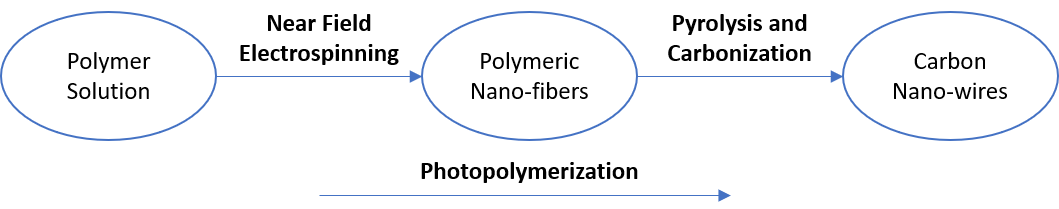
\includegraphics[width=0.95\textwidth]{./Figures/FabricationProcess.png}
%\decoRule
%\caption[Carbon Nano-wires Fabrication Process]{Fabrication process of carbon nano-wires to achieve through the proposed dissertation.}
%\label{fig:fabricationFlowChart}
%\end{figure}

%\begin{equation}
%\left(\tau _t^e-\frac{\tau _n^e \text{dr}}{\text{dz}}\right) 2 \pi  r+\frac{d \left(\pi  r^2
%   \left(\tau _{\text{zz}}-p\right)\right)}{\text{dz}}+\frac{\gamma  \text{dr} 2 \pi  r}{r
%   \text{dz}}+\rho  g \pi  r^2=\frac{d \left(\rho  \pi  r^2 v^2\right)}{\text{dz}}
%\label{eq:linearMomentum}
%\end{equation}
\chapter{Theoretical Framework} % Main chapter title

\label{Chapter:ConceptualFramework}

This section of the report provides with an overview of urban agriculture and its objectives with a theoretical framework of a sustainable city.

\section{Overview of urban agriculture}

The Food and Agricultural Organization defines urban agriculture as any production in the home or within urban area \cite{FAO2003}. In relation to the FAO definition of urban agriculture is the understanding that urban agriculture also implements the practices of farming and gardening in rural areas \cite{Opitz2016}. Some organisations limit their description of urban agriculture to gardens and farms within the inner city \cite{NewYorkN.Y..DepartmentofParksandRecreation.2010}, others include agricultural activities in the urban periphery area \cite{Mok2014}. Thebo, Drechsel, and Lambin \cite{Thebo2014} state a distinction between urban agriculture and urban periphery agriculture based on geographical location. Thebo et al. indicate that urban periphery agricultural activities take places within a distance of 10 to 20 $Km$ of the urban boundary. Based on Thebo's et al. distinction, the present paper addresses only agricultural activities that take place within an urban boundary. The work of Ayambire et al. \cite{Ayambire2019} gives a detailed distinction between urban and urban periphery agriculture.

The purpose of urban agriculture varies between cities. In the northern globe, people farm typically for recreational reasons although farming for household food supply \cite{McClintock2010}. In the southern globe, farming is mainly to satisfy household food needs and other commercial reasons \cite{Amponsah2016, McClintock2010}. Normally, households in the cities in the global south farm mainly for household consumption. On the other hand, rooftops, balconies and parks are used for agricultural purposes within the cities in the global north \cite{McClintock2010}. In this context, urban agriculture is implemented in this paper to study crop farming done through community gardens, backyard gardens and rooftops.

\section{Conceptualising a sustainable city}

The concept of sustainable cities originated in the United Nations World Commission on Environment and Development's (UNWCED) idea of sustainable development. The UNWCED summarised sustainable development as meeting the needs of the present generation without compromising the ability of future generations to meet their own needs. The concept has been a standard to address many areas of human activity. Sustainable cities determines the way humans shall interact with nature, as well as the way human shall take responsibility towards one another and future generations \cite{Yigitcanlar2015}. Lew, Ng, and Ni \cite{Lew2016} suggest that numerous definitions of sustainability and sustainable development are vague due to the varied understanding of sustainable development and the numerous definitions of sustainability \cite{Mebratu1998}. "Environmental economists believe in economic reductionism by undervaluing ecological goods while social ecologist is reductionist-holistic by focusing on the domination of people and nature." \cite{Mebratu1998} These lead to the separation of nature, economy and society, which is problematic for sustainability purposes. This report focus on sustainable development considers its tripartite dimension (economic, social and environmental).

The 11th SDG (Sustainable Development Goal) amplifies the sustainable city definition, which is “to make cities and human settlements inclusive, safe, resilient and sustainable. The concept is influenced by the rapid urbanisation of the world and the effects on the environment. The implication is that sustainability should be an imperative objective in every development plan. In this regard, the main goal of urban development shall be to make cities and ecosystems sustainable \cite{Hiremath2013}.

The compact city concept describes a city that is energy-efficient and less polluting due to the proximity of houses to the commercial areas and work places. The focus is on high density cities, which will result in less commute, efficient transportation and decreased emissions \cite{Abdullahi2015}. Typically, compact cities have less space for green-infrastructure due to the space limitations that have a negative effect on the quantity and quality of vegetation. Liu et al. have shown that compactness can have negative effects on domestic spaces, affordable shelter, and increased crime levels \cite{Liu2017}. These effects contradict the principles of a sustainable city, which target a balance among economic development, environmental protection, and equity in income, employment, shelter, services, infrastructure and transportation \cite{Hiremath}. For this reason, Garden Gem is not intended (but not limited) to be used within a compact city environment.

Models and indices are also based on conceptual terms. For that reason, the following lists the strengths and weaknesses of three indicators to measure a sustainable city. The use of indicators allow a detailed and quantitative way to measure sustainability within a city. This report reviews the existing models (the Green City Index, Global City Indicators Facility and the Global Compact Cities Circles of Sustainability) to develop a framework for a sustainable city. The framework intention id to serve as the basis for the role of urban agriculture in sustainable cities.

\subsection{The Green City Index}

The Green City Index is known as one of the robust models for the identification of a sustainable city \cite{Huang2015}. It comprises thirty indicators, grouped in eight categories. The categories comprise

\begin{itemize}
    \item Environmental governance
    \item Carbon dioxide (CO2)
    \item Buildings
    \item Transport
    \item Water
    \item Waste and land use
    \item Energy
    \item Air quality (refer to Appendix \ref{AppendixA}).
\end{itemize}

The benefits of this model is the ability to be applied in several geographical contexts. The index has been the implemented in the following reports: African Green City Index, Asian Green City Index, European Green City Index, German Green City Index, Latin American Green City Index, and U.S. and Canada Green City Index \cite{Huang2015}. The wide application of the model, its comprehensiveness and attribute as a “strong sustainability indicator” Huang et al. \cite{Huang2015}.

The indicators on carbon dioxide (CO2), which aims to reduce emissions, are directly linked to the indicators on transportation and air quality. The use of non-car transportation and increased use of green transport will most likely lead in the improvement of air quality. The indicators on energy are directly linked to the indicators on buildings. The management of energy consumption and the increase in the use of renewable energy are most likely to result in energy-efficient buildings.

\subsection{Global City Indicators Facility}

The Global City Indicators Facility attempts to include most aspects of urban cities, with a focus on economic and social matters (refer Appendix \ref{AppendixB}). The model defines a sustainable city based on its economic and social structures. The Global City Indicators Facility was created by the World Bank, working with the Japanese Trust Fund. Its weakness is the lack of focus on pollution, air quality, CO2 emissions, and renewable energy. Moreover, indicators on waste-water, water and particulate matter emissions are considered in the Global City Indicators Facility. The Global City Indicators Facility is designed to focus on cities with a population of over 100 thousand \cite{Mccarney2009}.

In another vein, the Green City Index and the Global City Indicators Facility agree on the use of specific indicators such as solid waste, transportation, waste-water, water consumption and energy. However, they do not cover aspects of food, flora and fauna. These are essential requirements for sustainable cities \cite{Ackerman2014, Opitz2016, Specht2014}.

\subsection{Global Compact Cities Circles of Sustainability}

The Global Compact Cities Circles of Sustainability is used to assess the sustainability in a city. It has been used by various cities such as Johannesburg, Melbourne, New Delhi, São Paulo and Tehran and by various organisations such as the UN Global Compact Cities Programme, World Vision and Save the Children to address sustainability efforts. The Global Compact Cities Circles of Sustainability is based on 28 indicators (refer to Appendix \ref{AppendixC}), which are categorized in four sub-categories.

The weaknesses of the Green City Index and the Global City Indicator Facility in not providing food flora and fauna measurements are covered by the Global Compact Cities Circles of Sustainability. An analysis of the Global Compact Cities Circles of Sustainability shows some similarities with the Green City Index and Global City Indicators Facility in regards to health, education, gender, technology, infrastructure, waste, water and air indicators. The indicators in the Global Compact Cities Circles of Sustainability are supportive. For example, reducing emissions and waste are prone to improve the habitat, settlements, recreation, identity of an area. Nevertheless, the Global Compact Cities Circles of Sustainability, unlike the Green City Index and the Global City Indicators Facility, does not address the environment, energy management and social engagement.

The report addresses a framework that merges the three indicators to measure sustainability in the three dimensions: economic, social and environmental. Figure \ref{fig:sustainableCityFramework} illustrates the combined framework presents the indicators that were used to assess the relation between urban agricultural and sustainable cities.

%\begin{figure}[th]
%\centering
%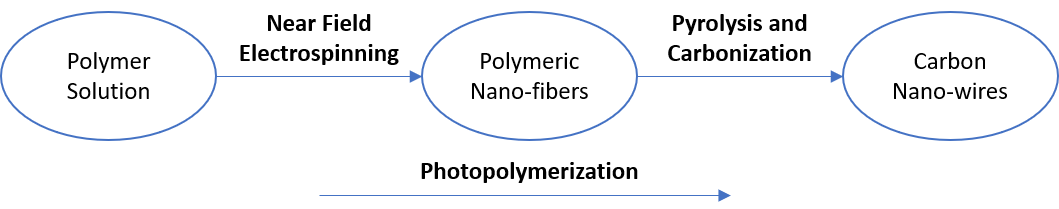
\includegraphics[width=0.95\textwidth]{./Figures/FabricationProcess.png}
%\decoRule
%\caption[Carbon Nano-wires Fabrication Process]{Fabrication process of carbon nano-wires to achieve through the proposed dissertation.}
%\label{fig:fabricationFlowChart}
%\end{figure}

%\begin{equation}
%\left(\tau _t^e-\frac{\tau _n^e \text{dr}}{\text{dz}}\right) 2 \pi  r+\frac{d \left(\pi  r^2
%   \left(\tau _{\text{zz}}-p\right)\right)}{\text{dz}}+\frac{\gamma  \text{dr} 2 \pi  r}{r
%   \text{dz}}+\rho  g \pi  r^2=\frac{d \left(\rho  \pi  r^2 v^2\right)}{\text{dz}}
%\label{eq:linearMomentum}
%\end{equation}
\chapter{Methods} % Main chapter title

\label{Chapter:Methods}

The study is based on a systematic review of secondary data. The term secondary data is used in this study to refer to data that are used to address research questions that are different from the ones the original collector sought to answer (Vartanian, 2011). The search for the secondary data was guided by phrases such as: a) urban agricultural practices, b) indicators for the measurement of sustainable cities, c) economic, social and environmental benefits of urban agriculture, and d) negative effects of urban agriculture on the city. At the end of the search, 189 articles/reports/books related to urban agriculture and sustainable cities were used.

The literature on indicators for sustainable cities was screened for commonalities and differences towards building a conceptual framework, which was used to analyse the nexus between urban agriculture and sustainable cities. The conceptual framework was developed from the following models: a) the Green City Index (Supplementary Table 1), b) the Global City Indicators Facility (Supplementary Table 2) and c) Global Compact Cities Circles of Sustainability (Supplementary Table 3). The framework integrates the strengths of each model and together addresses the inherent weaknesses of a single model. The indicators were then categorised into three, namely economic, social and environmental to reflect the concept of sustainable development (Fig. \ref{fig:sustainableCityFramework}). The three dimensions are referred to as themes in this article. The literature was analysed by subjecting each of the content analysed to the specific indicators under the sustainable city themes.

\begin{figure}[th]
\centering
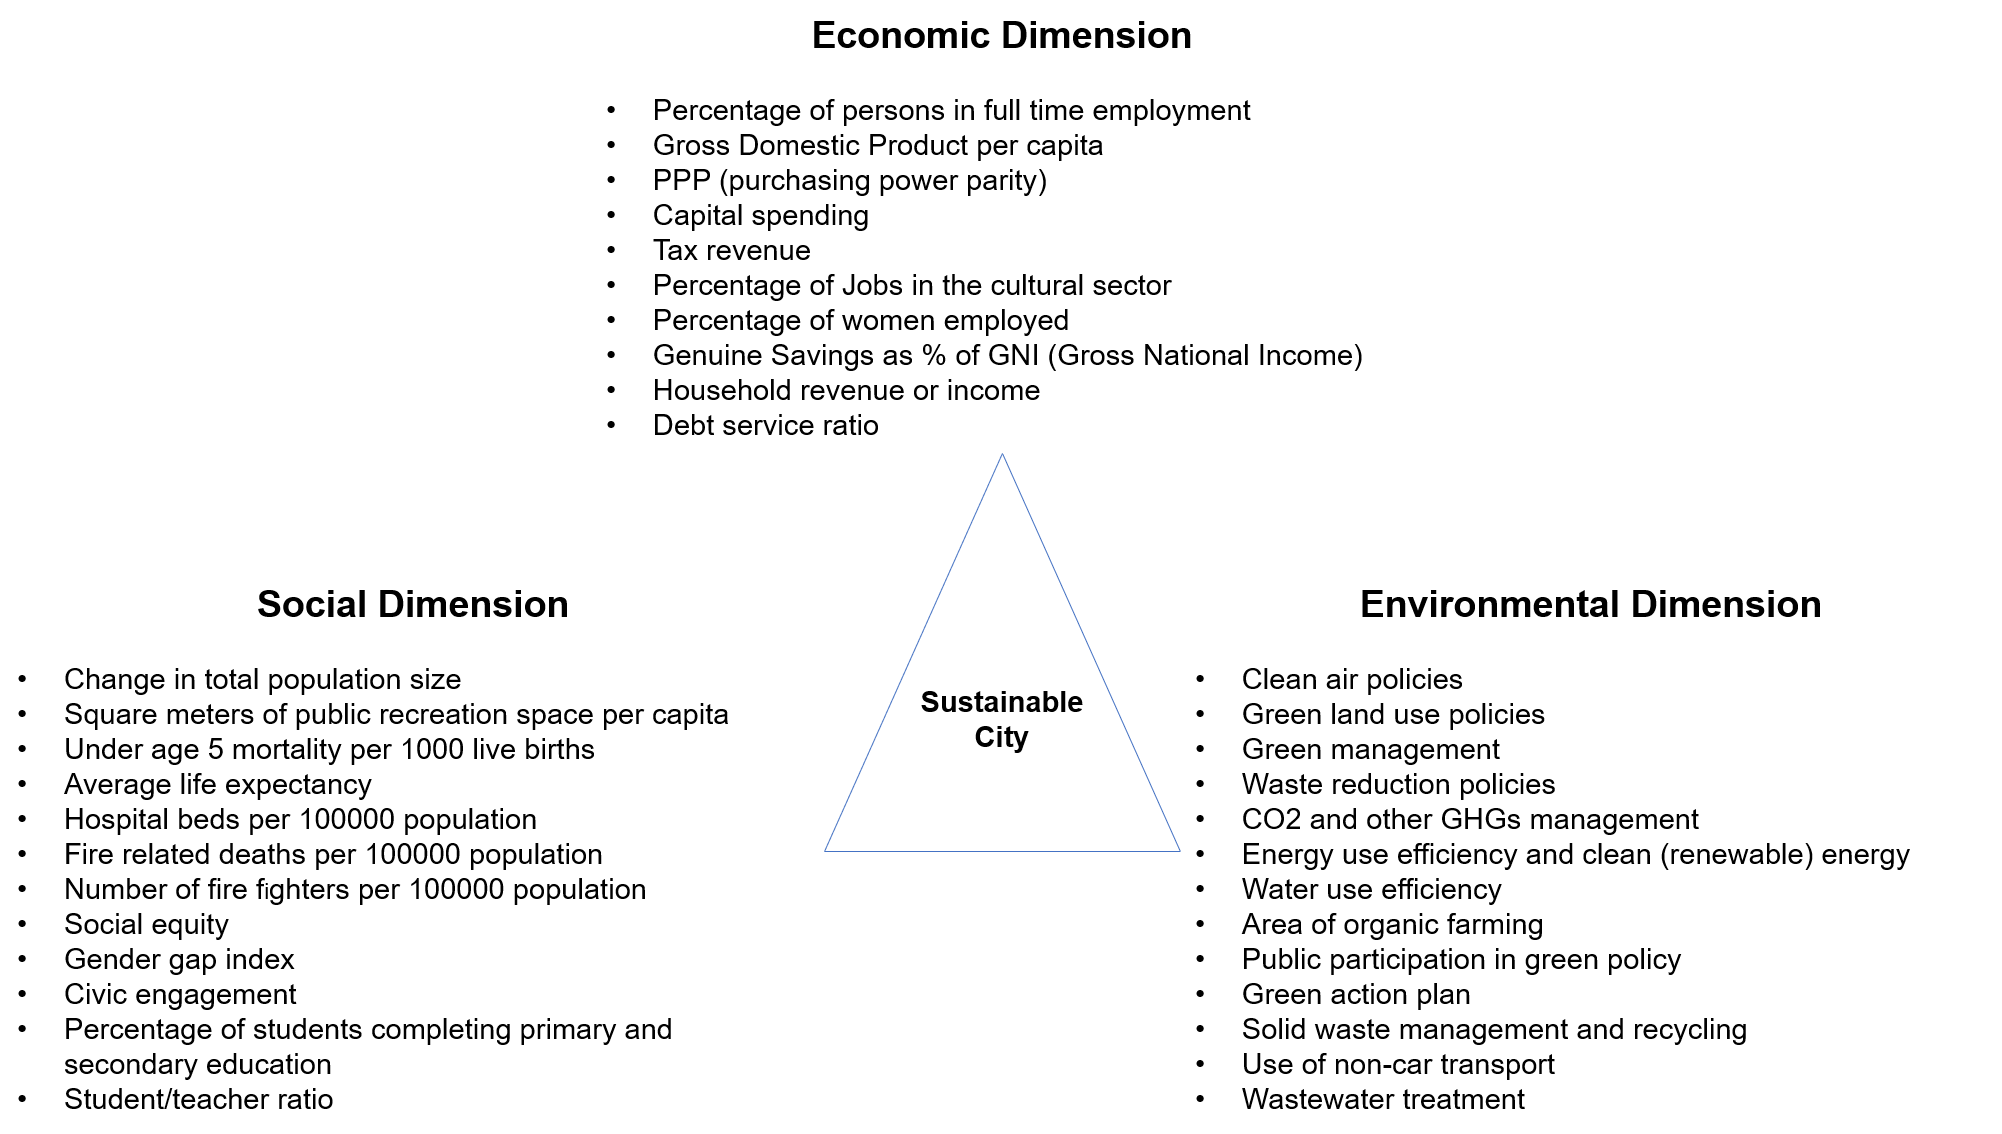
\includegraphics[width=1.00\textwidth]{./Figures/sustainableCityFramework.png}
\decoRule
\caption[Sustainable City Framework]{Sustainable City Framework.}
\label{fig:sustainableCityFramework}
\end{figure}

The literature was drawn from several geographical locations with different agro-climatic, economic, social and environmental characteristics. Lessons from these places underscore the importance of urban agriculture to the sustainable city discourse. For instance, in the global north, the importance of urban agriculture is more environmental in nature than socio-economic. However, the social and economic functions of urban agriculture are more pronounced in the cities in the global south. Despite these differences, the conceptual framework in the present study brings together economic, social and ecological indicators and can be applied in every city. The selection of the crops to cultivate to achieve the sustainability goals would however be based on the local climatic conditions.

%\begin{figure}[th]
%\centering
%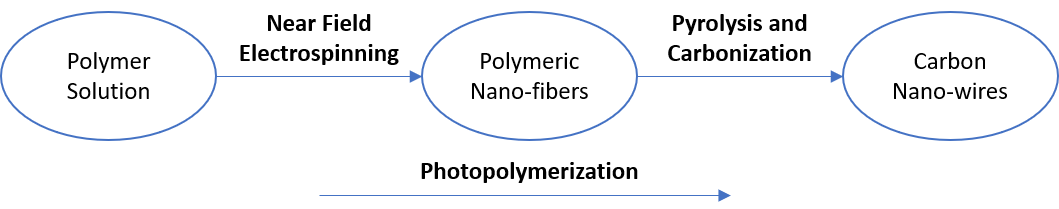
\includegraphics[width=0.95\textwidth]{./Figures/FabricationProcess.png}
%\decoRule
%\caption[Carbon Nano-wires Fabrication Process]{Fabrication process of carbon nano-wires to achieve through the proposed dissertation.}
%\label{fig:fabricationFlowChart}
%\end{figure}

%\begin{equation}
%\left(\tau _t^e-\frac{\tau _n^e \text{dr}}{\text{dz}}\right) 2 \pi  r+\frac{d \left(\pi  r^2
%   \left(\tau _{\text{zz}}-p\right)\right)}{\text{dz}}+\frac{\gamma  \text{dr} 2 \pi  r}{r
%   \text{dz}}+\rho  g \pi  r^2=\frac{d \left(\rho  \pi  r^2 v^2\right)}{\text{dz}}
%\label{eq:linearMomentum}
%\end{equation}
\chapter{Analyses} % Main chapter title

\label{Chapter:Analyses}

As presented in Fig. \ref{fig:sustainableCityFramework}, the indicators for measuring a sustainable city are categorised into economic, social and environmental. This section of the paper discusses the nexus between urban agriculture and sustainable cities with reference to the indicator-sets under each of the themes.

\section{Urban agriculture and economic sustainability of cities}

\subsection{Full-time employment}

Urban agriculture provides employment, and has thus become a major means of livelihood, for people in many cities particularly in the global south (Darkey et al., 2014; Zezza \& Tasciotti, 2010). An estimated 2100 farm labourers in Morogoro and 6400 in Mbeya, Tanzania are engaged in urban agriculture as either attendants or fodder collectors (International Labour Organization, 2013). Similarly, approximately 120,000 low-income households (including farmers, garland makers and garland sellers) in Manila, Philippines depend on jasmine production for their livelihoods (IPC, 2007). Many examples of urban agriculture's role in employment creation abound in the conventional literature (see: Amponsah et al., 2015a; Carr, Potter, \& Nortcliff, 2011; Sinclair, 2010; Tiongco, Narrod, \& Bidwell, 2010). The general observation is that urban agriculture's role in employment creation is widespread in the global south as depicted in Table \ref{tbl:peopleEngagedInUA}.

\begin{table}[th]
\caption{Number of people engaged in urban agriculture in the global south. Source: FAO (2007).}
\begin{center}
\begin{tabular}{ p{0.20\textwidth} p{0.25\textwidth} p{0.45\textwidth} } 
\hline
Region & Number (million) & Principal live-hood \\
\hline
Sub-Saharan Africa & 11 & Commercial vegetable growing or dairy farming \\
Northern Africa and the Middle East region & 6 & Horticultural and livestock products (fruit, vegetables and poultry) \\
South Asia & 11 & Perishable high-value commodities such as milk and fresh vegetables \\
East and South-East Asia & 7 & Perishable high-value commodities such as milk and fresh vegetables \\
\hline
\label{tbl:peopleEngagedInUA}
\end{tabular}
\end{center}
\end{table}

Not only is urban agriculture a source of employment to farmers but also to stakeholders along the value chain (Fig. \ref{fig:vegySupplyChain}). Community and farmers' markets and door-to-door delivery of food baskets in Argentina, Brazil and Uruguay are examples of jobs created in the commercial sector by urban agriculture (International Labour Organization, 2013). Similarly, majority of vegetable farmers in urban and peri-urban Ghana deliver their produce to wholesalers, who are predominately women, at the farm-gate (Abaidoo et al., 2009; Amoah, Drechsel, Henseler, \& Abaidoo, 2007; Amponsah et al., 2016). These wholesalers in turn sell the produce to retailers, food vendors and households as depicted in Fig. \ref{fig:vegySupplyChain}. The farm produce is conveyed from the farm-gate to the open markets by transport operators.

\begin{figure}[th]
\centering
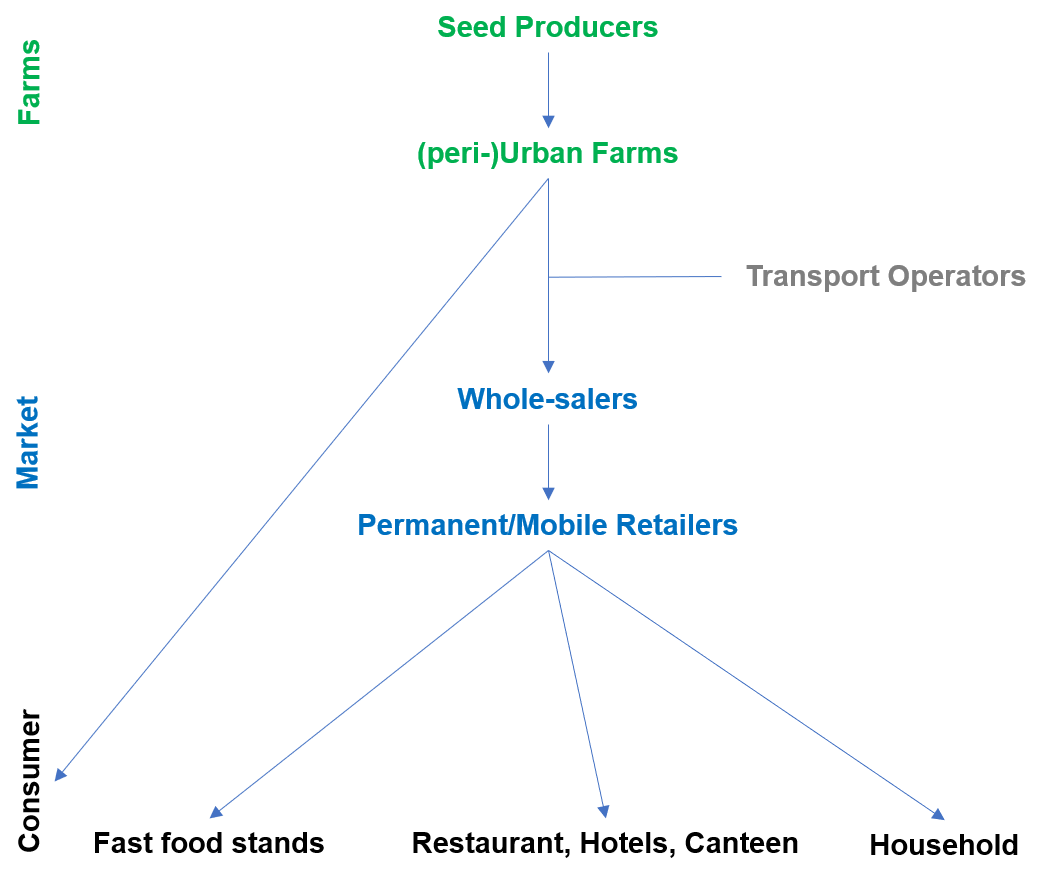
\includegraphics[width=0.75\textwidth]{./Figures/vegySupplyChain.png}
\decoRule
\caption[Carbon Nano-wires Fabrication Process]{Fabrication process of carbon nano-wires to achieve through the proposed dissertation.}
\label{fig:vegySupplyChain}
\end{figure}

The discussion so far suggests that urban agriculture makes a profound contribution to the employment of the labour force in the global south. The situation differs from the cities in the global north because the narrative in the conventional literature suggests that the motivation for urbanites and city authorities to promote agriculture in these cities lies in its ecological functions as well as its support for leisure and recreation (Pearson et al., 2010). The implication is that the role of urban agriculture in employment creation in the global north may not be as profound as it is in the global south. This is because, urban agriculture in the global north is not economically-centred but rather centred on its environmental functions. Nonetheless, recent studies give indications that the functions of urban agriculture in the global north is gradually shifting from leisure and recreation to more of urban sustainability and economic resilience (Lovell, 2010; McClintock, 2010). The increasing focus on economic resilience means that the contribution of urban agriculture in the global south and north appears to be converging even though there are variations across cities. Nevertheless, if the agricultural lands had been used for non-agricultural purposes, the employment effects may have been more profound. For instance, industrial and commercial activities on these parcels of land may have made more profound contributions to employment creation.

\subsection{Employment for women}

According to Prain and Lee-Smith (2010), two out of every three urban farmers in Yaounde, Nakuri, Maputo, Nairobi and Kampala are women. Generally, these women farmers engage in subsistence farming with the objective of meeting the family demand for fresh, nutritious and chemical-free food (Gamhewage, Sivashankar, Mahaliyanaarachchi, Wijeratne, \& Hettiarachchi, 2015). The rest of the urban women farmers sell the excess produce for income. However, agriculture could be a burden to these women due to the numerous roles they perform at the household level. The argument does not pertain to agriculture but also applies to almost all the economic activities the women are engaged in. The implication is that without addressing the issues that foster gender inequality, women's engagement in agriculture in the cities could be a burden (Veenhuizen, 2006). There must therefore be a conscious effort by policy makers and social advocates to help minimise the pressure on women emanating from the combination of household chores and economic activities such their involvement in urban agriculture.

Generally, commercial urban agriculture is dominated by men as depicted in Table \ref{tbl:genderinUA}. In contrast, women are dominant at the market and food vending stages of the supply chain (Drechsel \& Keraita, 2014). It can therefore be deduced that commercial agriculture in the cities in the global south is gendered and thus makes a profound contribution to employment for both women and men. However, as the economic arguments have always been, if the agricultural lands were used for nonagricultural purposes, more women may have been employed. This argument lies at the heart of the theory of ‘highest and best use’ of urban land.

\begin{table}[th]
\caption{Gender in urban agriculture in selected cities. Source: Drechsel et al. (2006).}
\begin{center}
\begin{tabular}{ p{0.20\textwidth} p{0.40\textwidth} p{0.15\textwidth} p{0.15\textwidth} } 
\hline
Country & City & Female (\%) & Male (\%) \\
\hline
Benin & Cotonou & 25 & 75 \\
Burkina Faso & Ouagadougou & 38 & 62 \\
Cameroun & Yaoundé & 16 & 84 \\
Cote d'Ivoire & Abidjan/Bouake & 5-40 & 60-95 \\
Gambia & Banjul & 90 & 10 \\
Ghana & Accra, Kumasi, Takoradi and Tamale & 10-20 & 80-90 \\
Guinea & Conakry, Timbi-Madina & 70 & 30 \\
Mali & Bamako & 24 & 76 \\
Mauritania & Nouakchott & 15 & 85 \\
Nigeria & Lagos/Ibadan & 5-25 & 75-95 \\
Sierra Leone & Freetown & 80-90 & 10-20 \\
Togo & Tsévié, Lome & 20-30 & 70-80 \\
India & Delhi, Mumbai, Chennai, Hyderabad and Bengaluru & 17 & 83 \\
\hline
\label{tbl:genderinUA}
\end{tabular}
\end{center}
\end{table}

\subsection{Income generation and gross domestic product}

Several households in both developing and middle income countries opt for urban agriculture as a source of livelihood (Abaidoo et al., 2009; Foeken \& Owuor, 2008; Raschid-Sally \& Jayakody, 2008a). Drechsel and Keraita (2014) point out that two out of every three urban vegetable farmers in Accra, Ghana had no intentions of leaving the job even if they were offered regular salaried employment. Based on this and many other factors (such as limited employment opportunities in the formal sectors, flexibility in work schedules, etc.), Amponsah et al. (2015b) conclude that vegetable farming in Kumasi, Ghana's second largest city, had become an employment destination for many.

Amponsah et al. (2015b) conclusion could be attributed to the higher incomes the farmers earned from the agricultural activities in the cities. For instance, Keraita, Jiménez, \& Drechsel (2008) identified that urban farmers in Ghana earned twice or more the incomes of their counterparts in rural areas. This appears to be the case in several other cities in the global south as indicated in Table \ref{tbl:incomesByUfarmens}. The earnings enable the urban farmers to contribute to national income. For instance, YiZhang and Zhangen (2000) found that 2.7 million urban farmers contributed 2\% of Shanghai's gross domestic product. Similarly, para grass production and sale in Hyderabad, India contributes an estimated annual income of USD 4.5 million to the city's economy. In Hartford, USA, urban agriculture is estimated to contribute between 4 and 10 million dollars in gross domestic product (Nugent, 1999).

\begin{table}[th]
\caption{Incomes earned by urban vegetable farmers in six cities. Source: Ensink et al. (2004); Buechler \& Devi (2005); Drechsel et al. (2006); Keraita, Jiménez, \& Drechsel, 2008.}
\begin{center}
\begin{tabular}{ p{0.30\textwidth} p{0.30\textwidth} p{0.30\textwidth} } 
\hline
City & Annual income per ha (US\$) & Annual GNI per capita (US\$) \\
\hline
Nairobi in Kenya & 1770 & 645 \\
Dakar in Senegal & 2234 & 773 \\
Kumasi in Ghana & 420-1920 & 522 \\
Hyderebad in India & 830-2800 & 771 \\
Haroonabad in Pakistan & 840 & 931 \\
Guanajuato in Mexico & 1935 & 7755 \\
\hline
\label{tbl:incomesByUfarmens}
\end{tabular}
\end{center}
\end{table}

The value of urban agriculture to a city's gross domestic product may not be significant when compared to non-agricultural land uses. This could be a justification for the pricing out of agriculture in city land use planning processes. However, as indicated earlier, gross domestic production and other economic indicators underestimate the actual contribution of urban agriculture to city development. The approach excludes ecological and social dimensions of urban agriculture. Probably, if these dimensions could be valued and added to the value of urban agriculture, then urban agriculture could be as valuable as other land uses.

\subsection{Savings and expenditure}

A study by Prain and Lee-Smith (2010) revealed that households who consumed the produce from their farms in Kampala in Uganda and Yaounde in Cameroon were able to save part of their incomes. Once individuals farm on their own, there is no need to spend money to buy some agricultural commodities. On this basis, Smit, Nasr, \& Ratta (2001) maintains that households who engaged in farming in cities in Zambia saved between 10 and 15\% of food costs. Furthermore, studies in Bangalore, Nairobi, Lima and Accra revealed that savings coming from own food production enabled households to purchase other types of food (World Bank, 2013). For instance, households in Bangalore were able to save between 1.30 and 80.00 USD per month (World Bank, 2013) whereas farmers in the cities in Kenya were able to save between 7 and 14 USD per month (Freeman, 1993). These savings are spent on other household items that contribute to improved quality of life.

It can be observed from Table \ref{tbl:expenditurePattern} that expenditure on food in Bangalore, Accra and Nairobi for households who engaged in urban agriculture was below the average of 50–70\% for the urban poor (FAO, 2007). The situation in the cities in the global north may be different given that urban households are driven by leisure and recreation to engage in agriculture cites. In these cities, households spend minimum proportions of their incomes on food, which implies limited contribution of urban agriculture to household savings. The savings may however originate from transportation. The literature indicates that households spend less on transport to obtain or transport food as compared to the other household items. Hamilton et al. (2013) had earlier observed that savings occurred as a result of the reduction in transport cost for the urban farmer. The savings result from the amount these farmers would have otherwise incurred if they were to travel to procure the items, they produce themselves. Furthermore, urban agriculture means some farm produce are now closer to consumers than if the produce were to be supplied by rural farmers. This will therefore reduce travel cost and time to access food items by urban dwellers.

\begin{table}[th]
\caption{Expenditure pattern of urban agriculture households in some selected cities. Source: World Bank (2013).}
\begin{center}
\begin{tabular}{ p{0.30\textwidth} p{0.20\textwidth} p{0.20\textwidth} p{0.20\textwidth} } 
\hline
Expenditure item & Selected cities &  &  \\
  & Bangalore & Accra & Nairobi \\
\hline
Food & 29.2 & 36.5 & 39.4 \\
Utilities & 16.8 & 12.3 & 13.1 \\
Education & 11.5 & 16.7 & 16.9 \\
Health & 10.4 & 8.2 & 5.1 \\
Clothes & 8.1 & 7.7 & 3.0 \\
Shelter & 7.0 & 3.2 & 18.9 \\
Loan/debt & 6.2 & 1.4 & 0.4 \\
Transport & 4.6 & 7.9 & 2.5 \\
Other & 3.3 & 0.8 & 0.2 \\
Family events & 2.1 & 4.5 & 0.2 \\
Domestic help & 0.7 & 0.8 & 0.2 \\
\hline
\label{tbl:expenditurePattern}
\end{tabular}
\end{center}
\end{table}

\subsection{Tax revenue}

Taxes are very important elements in managing developmental activities in cities. Taxes collected through urban agriculture covers all the actors along the produce supply chain. It is worth noting that, national income from taxes from urban agriculture can be directly linked to the expenditure farmers make and the employment obtained.

Property taxes have been identified as a city's main source of income (World Bank, 2015). Urban agriculture contributes significantly to tax revenues from property taxes. According to Liu (2008) and Voicu and Been (2008), urban farms and community gardens contribute to the increase in home values. For instance, the presence of gardens in California contributed to the rise in property values as much as 9.4% within five years of establishment (Voicu & Been, 2008). The revenues were estimated at half a million dollars per garden over twenty years.

Transportation taxes are also paid by urban farmers who transport their goods within or outside the urban area. Some urban farmers indirectly pay transportation taxes through the purchase of fuel for irrigation or the transportation of farm goods and services. Additionally, the wholesalers or retailers engaged in the sale of the urban agricultural produce pay taxes to city authorities. In Kumasi, a city in Ghana, wholesalers and retailers who operate in the open markets pay taxes in the form of market tolls (tickets) (Baah-Ennumh \& Adom-Asamoah, 2012). The amounts paid ranges from 5 to 10GHp (0.01 USD–0.02 USD) a day and are paid to the Kumasi Metropolitan Assembly. Similarly, in the United States, the income that is obtained from urban farming does not represent a separate kind of income. They are determined and taxed like income from other businesses of a comparable size apart from some detailed regulations regarding farm income. However, national subsidies for soil, groundwater or environmental protection, care for wild animals or forests are sometimes tax-free for the farmers (Andersen, Asheim, Mittenzwei, \& Veggeland, 2002). In a similar vein, some municipalities (Rosario in Argentina and Cagayan de Oro in The Philippines) use tax exemptions as a means of promoting urban agriculture.

Useful as the taxes may be, taxes to the cities may be more if the agricultural lands had been used for non-agricultural purposes such as commerce or industry. The tax exemptions could also be avoided if the lands were used for non-agricultural purposes. Such arguments are underpinned by the theory of ‘highest and best use’ which focuses on only the direct economic benefits derived from the use of land. These theories suggest that allocating land for urban agriculture deprives its access for other more economically beneficial uses such as industrial, commercial and residential uses. This explains why a rise in the value of urban agricultural land is mostly associated with the change in use from agriculture to alternative land uses (Nugent, 2000).

\section{Urban agriculture and social sustainability of cities}

\subsection{Educational functions}

Golden (2013) suggests that urban agriculture provides a medium for learning experiences, youth development and educational programmes. Agricultural projects in California and Philadelphia in the United States of America are used to highlight the role of urban agriculture in education (Bradley \& Galt, 2014; Ober Allen, Alaimo, Elam, \& Perry, 2008; Travaline \& Hunold, 2010). These educational services are directed towards teaching the citizens where, how and by whom the food they eat is grown so as to enable them make informed decisions about their food systems. The agricultural projects in the cities serve as avenues for children and adults to acquire practical skills on food production and processing.

Furthermore, through their social networks, urban farmers who have had the benefits of education by research institutions impart the knowledge to their counterparts. For instance, urban vegetable farmers in Kumasi in Ghana who have participated in research activities on the World Health Organization's Multiple Barrier Interventions have transferred the knowledge to their counterparts who were not part of the training programme (Amponsah, Vigre, Schou, Braimah, \& Abaidoo, 2015a). This is used to highlight the replication effects of such research projects on the larger community.

Urban farmers' earnings from agriculture are used to support their children in school (Prain \& Lee-Smith, 2010). A study conducted in SriLanka by Gamhewage et al. (2015) concluded that 22\% of urban farmers prefer to expend their savings on the education of their children to spending on household possessions. Similarly, in India, some women contribute approximately 23\% of their share in household education expenditure from the incomes they earn from urban agricultural activities. Another study in Kampala, Uganda also concluded that urban male farmers and female farmers spend 26\% and 12\% of their incomes respectively on the fees of their wards in school (Devi \& Buechler, 2009).

Nevertheless, urban agriculture, particularly in the global south, is known to fuel child labour and truancy in school (Edet \& Etim, 2013; International Labour Organization, 2006). For instance, in Dar es Salaam, Tanzania, children have been found to engage in urban agriculture at the expense of their education. Similarly, child migrants have been found to be engaged as farm labourers on urban farms in Kumasi, Ghana (Amponsah et al., 2016). Yet, in these countries, child labour is prohibited. The higher returns from the urban agricultural activities could be an explanation for their attractiveness to children, especially migrant children.

By enforcing the child labour laws, the children can take advantage of the free and compulsory universal primary educational policies and programmes in these countries to enrol in schools (Nishimura \& Yamano, 2013; Rodeghier, Hall, \& Useem, 1991). This will ultimately enhance the educational functions of urban agriculture towards social sustainability of cities.

\subsection{Civic engagement}

A growing body of literature points to the increasing importance of community supported agriculture in civic engagements. For instance, Obach and Tobin (2014) and Pole and Gray (2013) found that people in New York City who were engaged in urban agriculture were more politically engaged and more likely to volunteer in their communities compared to the general population. Similarly, in Dar es Salaam in Tanzania, urban farms were used as political gathering spaces in the run up to the 2010 elections. In fact, some farms had small concrete platforms that were used for political rallies. Despite these observations, Pole and Gray (2013) maintain that generally, the desire for organic foods is the motivation for people to interact with urban farmers other than civic engagement. Obach and Tobin (2014) add that consumers of urban agricultural produce are less likely to engage in charitable giving than the general population. The authors conclude that if the motivation for engaging in urban agriculture is economic, then it is less likely to promote civic engagement.

The narrative points out that economic reasons including household food security, employment and income generation are the main motivations for people's engagement in urban agriculture (Abaidoo et al., 2009; Amoah et al., 2007; Amponsah et al., 2016; Darkey et al., 2014; International Labour Organization, 2013; Zezza \& Tasciotti, 2010). On the other hand, the reasons for agriculture in the cities in the global north are more inclined towards leisure and ecological functions (Hamilton et al., 2013; International Labour Organization, 2013; Walker, 2015). In this regard, urban agriculture's role in civic engagement may be more pronounced in the global north than the global south.

\subsection{Safety and security}

Urban agriculture makes an important contribution to the safety of a city. For instance, roof-top gardens help to promote energy efficiency in buildings and contribute to fire prevention (Hoornweg & Munro-Faure, 2012; Rashid & Ahmed, 2011; Wong et al., 2003). Furthermore, clearing an area of bush in a city for agricultural purposes has the potential to eliminate hiding spaces for thieves (real or imagined). Customers, people walking through, people who live nearby, people looking for a day labour job, and more, all interact with urban farmers. The interactions make profound contributions to the social sustainability of cities.

A study by the University of Pennsylvania's Perelman School of Medicine in Philadelphia found that greening vacant lots (which could take the form of urban agriculture) made nearby residents feel significantly safer, and that the greened lots were linked to reductions in certain gun crimes in the area (Krauser, 2012). This is consistent with the results of the work of Kuo and Sullivan (2001) which revealed that the greener a building's surroundings were, the fewer the reported crimes. Following this, the Youngstown Neighbourhood Development Corporation initiated a ‘Lots of Green’ programme in 2010 to reuse vacant lands. A recent study established that there were reductions in burglaries around stabilisation lots, and assaults around community reuse lots (Kondo, Hohl, Han, & Branas, 2016). This could be a validation of the broken window theory, which states that maintaining and monitoring urban environments in a well-ordered condition may stop further vandalism and escalation into more serious crime. The Urban Food Crisis (2018) explains that using blighted lots for urban agricultural purposes sends a signal that criminal activities are not welcome in the area, which ultimately reduces crime rates.

Other studies point to the negative side of urban green space (Bixler & Floyd, 1997; Ulrich, 1993; Van den Berg & Ter Heijne, 2005). These include encounters with physical danger such as poisonous animals and thorny plants, and the fear of crime (Sreetheran & van den Bosch, 2014). These authors, after a systematic review of literature, point out, however, that factors such as gender and individual's experiences are most influential in evoking fear of crime. This means that the crimes that result from urban agriculture may be imagined from an earlier experience. A fear of crime may therefore be imagined but not real. People should be alerted to thorny plants and poisonous animals to mitigate the adverse effects on neighbourhoods. These measures could enhance the role of urban agriculture in urban safety and security.

\subsection{Gender equality and social equity}

Urban agriculture contributes to bridging gender gap and promotes social equity through the employment opportunities it offers to both men and women. As presented earlier in Table 2, women form a significant part of the labour force that is engaged in urban agriculture. They can gain employment at every stage of the supply chain. This reduces gender inequalities (Eigenbrod & Gruda, 2015; International Labour Organization, 2013). A study conducted in Kisumu in Kenya by Mireri (2013), concluded that the proportion of male family labour engaged in urban agriculture is slightly higher (53%) than that of women. However in the case of hired labour, more women (54%) than men were employed. Kutiwa, Boon, and Devuyst (2010) also point out that urban agriculture in Harare in Zimbabwe provides women the opportunity to earn secondary income, improve nutritional value of the household diets, and participate actively in budgeting and decisionmaking processes at the household level. Similarly, both men and women are engaged in mushroom production, horticulture, aquaculture and livestock farming in Accra in Ghana (World Bank, 2013). These cases reveal that urban agriculture contributes to bridging the gender gap, which has positive implications for social equity.

However, women tend to engage in urban agriculture for household food supply while men engage in it for economic reasons. This could perpetuate the income gap between men and women in many cities. Furthermore, the disparity in the gender roles at the family level implies greater burden on women in the cities in the global south than men. Typically women shoulder more household responsibilities (like childcare and domestic work) than men (Lachance-Grzela & Bouchard, 2010; Mencarini & Sironi, 2012), which implies that urban agriculture could have the potential to aggravate the burden of work on women and gender inequality (Veenhuizen, 2006). These have implications for the systems and practices that perpetuate gender inequality but not necessarily preventing a certain gender category from engaging in urban agricultural activities or any economic activities.

\subsection{Health benefits}

Urban agriculture contributes to the health of a city through its contribution to food security (Golden, 2013; Opitz et al., 2016; Twiss et al., 2003; World Bank, 2013) and income for farmers and their families to access health care. Community gardens give residents access to fresh fruits and vegetables (Larsen & Gilliland, 2009; Park et al., 2011), which are critical to safeguarding their health and that of the city in general. From a social point of view, urban agriculture can ensure food availability and accessibility, which can translate into food affordability. Also, women take advantage of the produce from household gardens to diversify the family food intake, which ultimately results in healthier diets. Research also shows that people who participate or have family members that engage in community gardens “were 3.5 times more likely to consume fruits and vegetables at least 5 times per day than people without a gardening household member” (Alaimo, Packnett, Miles, & Kruger, 2008). In this regard, urban agriculture helps to reduce malnutrition and promote the general health of the city population.

However, some studies point to the adverse effects of urban agriculture on the health of the cities. These studies highlight the excessive use of agro-chemicals (Obuobie et al., 2006; Veenhuizen, 2006; Yamusa, 2014), which could undermine the health of producers, consumers and environment at large, and the use of untreated wastewater for food production without regard to safe practices in many cities in the global south (Amponsah, Vigre, Schou, Braimah, & Abaidoo, 2015a; Becerra-Castro et al., 2015; Mara & Sleigh, 2010; Ndunda & Mungatana, 2013; Veenhuizen, 2006). In addition, the urban agricultural farms can result in the spread of diseases through mosquitoes and the scavenging animals.

Based on these adverse effects, the emphasis of the discourse on the role of urban agriculture in cities' social sustainability should focus on responsible agriculture. This underscores the need to regulate the urban agricultural subsector for compliance with safe agricultural practices and general neighbourhood sanitation measures.

\subsection{Recreation}

Community gardens and rooftop gardens contribute to both indoor and outdoor recreation (see Hamilton et al., 2013; Walker, 2015). These gardens can provide a place where people in an area in a city come together for mutual benefits. For instance, in the early 20th Century, upper class Russians resorted to dachas as hobby farming to improve upon recreation (Hamilton et al., 2013). Community gardens and rooftop garden also serve as tourist attraction centres (International Labour Organization, 2013) and improve the value of urban property. A classic example of this is in Beijing China. Here, people spend one-day to tour over 1900 sightseeing farms and pick produce (International Labour Organization, 2013).

Some individuals in Detroit have resorted to urban agriculture as a means of increasing the value of their property (Walker, 2015). Each community garden in California also contributed about half a million dollars to the local economy through rise in the value of real property (Voicu & Been, 2008). People are attracted to some of these buildings because of the plants and ornaments around. It is on the basis of this that the World Bank (2013) suggest that countries should consider integrating urban agriculture into urban greening as a means to improving recreation, aesthetics and property values in their cities.

\subsection{Technology and innovation promotion}

Urban agriculture provides the avenue for the development of technology. For instance, some urban farms in Hong Kong Island, China are recycling water with PV-powered UV-LED disinfection (Close, Ip, & Lam, 2006). Other farms use hydroponic (Buehler & Junge, 2016; VOA News, 2016; Woodford, 2018), film farming (Joe, 2017) and aeroponic (Vyawahare, 2016) systems to produce leafy greens, tomatoes, and herbs. These technologies could contribute to the preservation of urban agriculture and its significant roles even in cities where land is increasingly becoming scarce due to rapid urbanisation.

Urban agriculture also provides an avenue for new research and technology to be developed. Examples include research on varieties of seeds, and type and amount of light required for plant growth. This type of agriculture therefore incorporates the use of technology as a means of optimising levels of production. Disregarding technology and innovation in urban agriculture could result in unreliable and ineffective farms.

\section{Urban agriculture and environmental sustainability of cities}



%\begin{figure}[th]
%\centering
%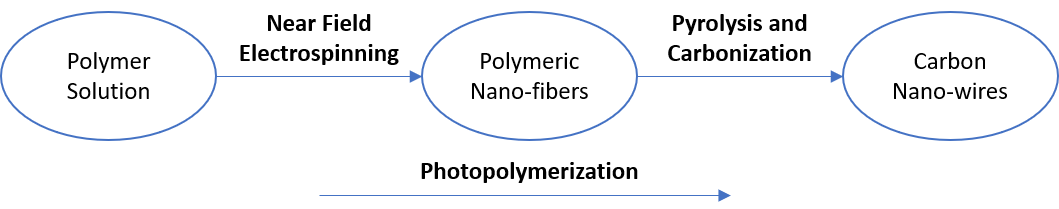
\includegraphics[width=0.95\textwidth]{./Figures/FabricationProcess.png}
%\decoRule
%\caption[Carbon Nano-wires Fabrication Process]{Fabrication process of carbon nano-wires to achieve through the proposed dissertation.}
%\label{fig:fabricationFlowChart}
%\end{figure}

%\begin{equation}
%\left(\tau _t^e-\frac{\tau _n^e \text{dr}}{\text{dz}}\right) 2 \pi  r+\frac{d \left(\pi  r^2
%   \left(\tau _{\text{zz}}-p\right)\right)}{\text{dz}}+\frac{\gamma  \text{dr} 2 \pi  r}{r
%   \text{dz}}+\rho  g \pi  r^2=\frac{d \left(\rho  \pi  r^2 v^2\right)}{\text{dz}}
%\label{eq:linearMomentum}
%\end{equation}
\chapter{Garden Gem} % Main chapter title

\label{Chapter:OurContribution}

Plentiful, healthy, economic and safe food for the entire planet is a topic to be held in our minds for the following years. Food safety and security are the main challenges to be discussed along with the confrontations against climatic change. At least 55\% of the world’s population already lives in urban areas, and this number is expected to rise to 65\% by 2050. (FAO, 2019) Nearly 80\% of all food produced is consumed in these urban areas and, according to information of the Food and Agriculture Organization of the United Nations, 60\% of irrigated and 35\% of rainfed croplands are within a 20 km radius of urban agglomerations. (FAO, 2019) Additionally, almost one third of all food produced for humans is lost into waste that comprises more than 50\% of all municipal waste. (FAO, 2019) Finally, it is important to point out that in low-income countries, food expenditures can take up to two thirds of the total household. (FAO, 2019) Food policies require training citizens about new lifestyles. The training purpose is to incentivize awareness to address sustainable food safety and security. (Sandrini, 2014)
The lifestyle of human kind shall be amended, particularly in regards of our food supply chain, from the farming, distribution to the end consumer. Through food education, the system players (consumers and producers) are trained. A new lifestyle will also have an environmental impact related to transportation and distribution. (Sandrini, 2014)

It is important to conserve farming land, especially in areas already subject to strong urbanization. GardenGem’s purpose is to be a tool for urban gardeners, researchers and citizens for food education and urban agriculture.

\section{Impact on the Economic Dimension}

Urban gardening has been part of the human economic activities since the emergence of cites as the urban phenomena developed. (Calvet-Mir, L., \& March, H., 2019) A study carried out by Calvet-Mir, L. \& March, H. established the importance of urban gardening as a response to financial crisis and their strong correlation to community resilience against war and other adversities. Populations of growing poverty rates in cities are also impacted by the development of urban gardens. Self-production or self-sufficiency of food are directly related to food security during economic crisis and shortages. Helping build self-sufficient cities improves the health and quality of food and rises awareness around local produce food sovereignty.

As detailed in Section \ref{sec:economicDim}, GardenGem takes this perspective into account, trying to aim towards an economically sustainable activity that can provide better food prices and optimal operational costs to any user of the application.

\section{Impact on the Social Dimension}

Urban gardening comes as a response to changing social and political circumstances. There have been numerous initiatives to promote their practice during conflicts and economic crisis to tackle food distribution problems during specific historical moments. These factors have an important effect shaping the form, function and culture of urban gardens and their members \cite{Calvet-Mir2019}. Since the last century, we have witnessed a growing institutional recognition of urban gardening, through national and local legislation in many countries, including Mexico.

Urban gardening portrays emancipatory and alternative views about the urban development and social relations. There is evidence of urban gardens being used to protest against political corruption, empowering the people and appealing to citizen responsibility to overcome any crisis \cite{Certoma2015}. Social entrepreneurship and social innovation are strongly related to urban gardening since it is subject of continuous improvement mainly due to the huge positive impact it has in people’s lives. It has been demonstrated that urban gardens have the effect of strengthening community ties, enabling intercultural exchanges, facilitating community building as and enhancing social cohesion where the garden is located \cite{Calvet-Mir2019}.

The GardenGem team is making research on these aspects to develop the right campaign for the encouragement of urban agriculture. We are working to find the correct approach towards people and government for incentivization and support. Section \ref{sec:socialDim} lists the social impact that Garden Gem is targeting.


\section{Impact on the Environmental Dimension}

Human beings have been altering their environment since the beginning of their existence; in fact, this specific trait is the most concluding evidence of human presence in any place or time. Urban planning is the practice of spatial arrangement of urban areas \cite{Certoma2015}. These arrangements unequivocally have an impact on the environment, thus the planification of cities must always consider alternatives for the best land distribution to allow human development without strangling itself by damaging its resources. Urban agriculture enhances the diversity and distribution of food and non-food products through processes that reuse human and material resources. This has a positive impact in and around the urban area supplying products and services to the same area in return \cite{Broadway2009}.

We want to prepare people with tools that empower them to take their environmental impact on their hands and start acting positively in the right direction. GardenGem is meant to improve the caring of the environment in a sustainable and practical way, by impacting the processes in Section \ref{sec:environmentalDim}.

\section{Garden Gem Objectives}

GardenGem is a mobile application that will help urban gardeners by assisting them in the correct development and maintenance of their urban gardens. Garden Gem’s will provide the information required to find compatible food plants with similar care and know the number of plants that can be placed within a given land area. Additionally, it will offer an in-app store to facilitate the purchase of materials and supplies for the optimal development of their urban garden. Further into the future, the app will feature a community intercommunication between urban gardeners to allow sharing and trading. The compatibility with other technologies as the Food Computer from the Open Agriculture Iniciative from the MIT will make this application even more useful for the automation of urban garden production.

Economical goal: To enable the average citizen, and local community to grow vegetables locally in order to save money and create a possible source of income. 

Social goal: To promote social integration and combat poverty by the creation of urban garden communities based on participation.

Environmental goal: To enhance the diversity and distribution of food products through processes that reuse resources in a sustainable and local way.

\subsection{Monetization}

The monetization of this product will be based in the in-app store where users and suppliers will receive small fees for each buy. One product that is expected to become a popular purchase is the kit for the construction of a Food Computer, since all the manuals and designs are openly available in the Open Agriculture Initiative. These fees will be the main source of income in the beginning. Once the community functionality is ready, trading fees between gardeners and direct consumers or distributors will support the application and its growth.

\section{Garden Gem Results}
\subsection{Development of the mobile application}

\begin{figure}[th]
\centering
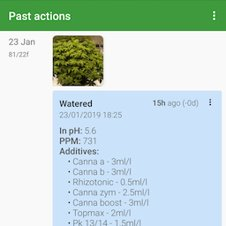
\includegraphics[width=0.45\textwidth]{./Figures/app1.png}
\decoRule
\caption[Record of the actions done to a given plant]{Record of the actions done to a given plant}
\label{fig:app1}
\end{figure}

\begin{figure}[th]
\centering
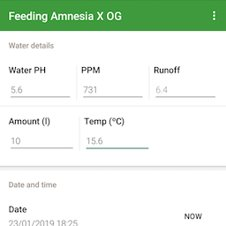
\includegraphics[width=0.45\textwidth]{./Figures/app2.png}
\decoRule
\caption[Feeding Amnesia X OG, characteristics]{Feeding Amnesia X OG, characteristics}
\label{fig:app2}
\end{figure}

\begin{figure}[th]
\centering
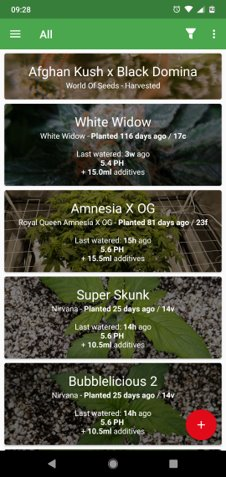
\includegraphics[width=0.45\textwidth]{./Figures/app3.png}
\decoRule
\caption[All plants]{All plants}
\label{fig:app3}
\end{figure}

The application can record data about growing plants in order to monitor the growing conditions and make the plants grow better by identify potential issues during the growing process. The application is also concentrating in the three pillars of sustainability focusing on its impact in the improvement of life standards for any user of our application according to the economic, environmental and social perspectives that were previously described in this project.

Figures \ref{fig:app1}, \ref{fig:app2} and \ref{fig:app3} show the final application running on an android device. In Figure 1 the actions that have been already done to the plant are recorded and showed. Figure 2 shows the proper characteristics needed for feeding Amnesia X OG. Finally, figure 3 shows all the current plants that are intended to growth in the best possible way.

According to the surveys performed to people from multiple backgrounds, the application received an approval rate of above 95\%. More than 60\% of the people who participated on the survey were already considering urban gardens before checking our app, and more than 90\% thought it would be useful. The complete results of this survey are presented in the annex section of this document.

%\begin{figure}[th]
%\centering
%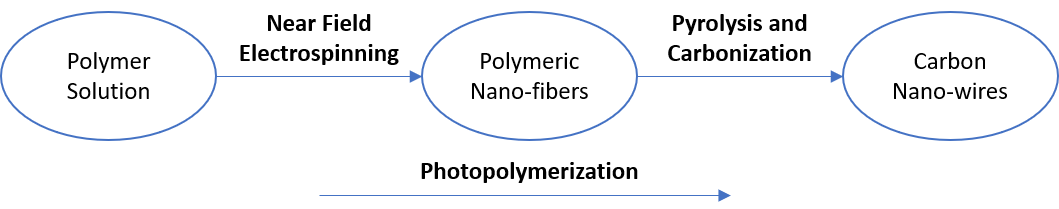
\includegraphics[width=0.95\textwidth]{./Figures/FabricationProcess.png}
%\decoRule
%\caption[Carbon Nano-wires Fabrication Process]{Fabrication process of carbon nano-wires to achieve through the proposed dissertation.}
%\label{fig:fabricationFlowChart}
%\end{figure}

%\begin{equation}
%\left(\tau _t^e-\frac{\tau _n^e \text{dr}}{\text{dz}}\right) 2 \pi  r+\frac{d \left(\pi  r^2
%   \left(\tau _{\text{zz}}-p\right)\right)}{\text{dz}}+\frac{\gamma  \text{dr} 2 \pi  r}{r
%   \text{dz}}+\rho  g \pi  r^2=\frac{d \left(\rho  \pi  r^2 v^2\right)}{\text{dz}}
%\label{eq:linearMomentum}
%\end{equation}
\chapter{Conclusion} % Main chapter title

\label{Chapter:Conclusion}

%\begin{figure}[th]
%\centering
%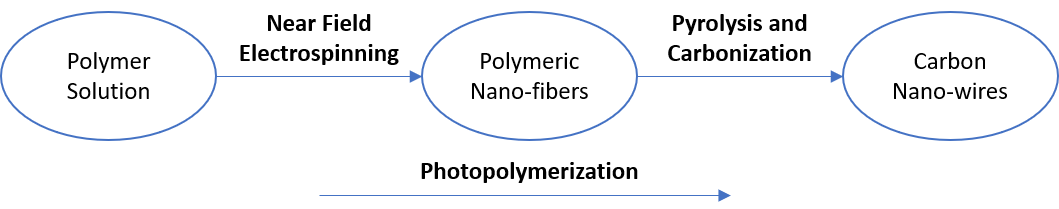
\includegraphics[width=0.95\textwidth]{./Figures/FabricationProcess.png}
%\decoRule
%\caption[Carbon Nano-wires Fabrication Process]{Fabrication process of carbon nano-wires to achieve through the proposed dissertation.}
%\label{fig:fabricationFlowChart}
%\end{figure}

%\begin{equation}
%\left(\tau _t^e-\frac{\tau _n^e \text{dr}}{\text{dz}}\right) 2 \pi  r+\frac{d \left(\pi  r^2
%   \left(\tau _{\text{zz}}-p\right)\right)}{\text{dz}}+\frac{\gamma  \text{dr} 2 \pi  r}{r
%   \text{dz}}+\rho  g \pi  r^2=\frac{d \left(\rho  \pi  r^2 v^2\right)}{\text{dz}}
%\label{eq:linearMomentum}
%\end{equation}

%\chapter{Introduction} % Main chapter title

\label{Chapter:Introduction}

Globally, urban land attracts very high rent. This is attributed to rapid urbanisation and ease of accessibility \cite{Trussell2010}. Consequently, farmers who are unable to compete for lands due to their low bid rents, have been priced out of the urban land market \cite{Amponsah2015, Amponsah2016, Keraita2008, Owusu2012}. This is the central position of the William Alonso's bid-rent theory. The theory explains how land users are willing to pay high rents for an area of land in an open and competitive land market. Similarly, the theory of ‘highest and best use’ has been used to justify the allocation of city lands to uses that command high bid rent \cite{Scholz1933, Barkley1986, Fisher1954}. The theory expresses the need to allocate city land to uses that produce the largest net income over a given period of time \cite{Fisher1954}. Therefore, city authorities give prominence to nonagricultural uses on the scale of city land allocation preference. Consequently, agriculture has been confined to the urban periphery and rural areas where the value of land is within the means of agricultural land users.

However, rapid urbanisation and its attendant sprawl, particularly in the global south, are threatening the sustainability of agriculture even at the urban periphery \cite{Amponsah2015, Liu2017}. Projections by the United Nations indicate that by 2020, the developing countries of Africa, Asia and Latin America will be home to approximately three in four urbanites, and eight of the anticipated nine mega-cities in the world. Furthermore, by 2030, approximately twothirds of the world's population will live in cities. The expected increases in the city population will have implications for high demand for urban lands leading to their allocation to the highest and best use. Furthermore, agricultural land uses in the urban periphery will continue to be invaded by the more competitive land uses, which could have dire consequences on food security and poverty levels \cite{Hoornweg2012}.

From the discussion, urban agriculture can only be sustained if city authorities consciously integrate agriculture into the city land use planning and zoning processes. Nevertheless, the city authorities, particularly in the global south, have given little to no attention to agriculture despite their resolve to make their cities sustainable (evident in the Sustainable Development Goal 11). This could be explained by their apparent belief that the highest and best use of city land is not to allocate it to agricultural uses. This belief may have been fuelled by the lack of clarity in the narrative in the conventional literature about the role of urban agriculture in building sustainable cities. The literature on the effects of urban agriculture is contested between two divides. The first maintains that agriculture in cities performs economic, social and environmental functions, which contribute to the sustainability of cities. For instance, agriculture in cities in Sub-Saharan Africa supplements the nutritional needs of urbanites and reduces their food expenditure \cite{Binns2013}. In Yaounde in Cameroon, urban farmers consume almost a quarter of the vegetables they produce \cite{Prain2010}, whereas in Ghanaian cities, urban vegetable farmers supply almost all the exotic vegetables (lettuce and spring onion) that are consumed in the cities \cite{Kodjo2014, Drechsel2014}. The works of Ackerman et al. \cite{Ackerman2014}, Opitz et al. \cite{Opitz2016}, Specht et al. \cite{Specht2014} and Ayambire et al. \cite{Ayambire2019} also highlight the role of urban agriculture in food security.

Besides the economic functions, urban agriculture is known to perform social and environmental functions. The environmental functions are in the forms of air and water quality enhancement (Lin, Philpott, \& Jha, 2015), and pollination and biocontrol activities (Camps-Calvet, Langemeyer, Calvet-Mir, \& Gómez-Baggethun, 2015; Lin et al., 2015). The social functions are evident in its support for political activism and volunteerism in cities. For example, a study showed that farmers in New York City are more likely to engage in voluntary works for community development than the general population (Obach \& Tobin, 2014; Pole \& Gray, 2013). Also, farms in Dar es Salaam in Tanzania serve as rallying grounds for political parties during election years (McLees, 2016). Dimitri et al. (2016) note that urban farms provide educational and community building functions (e.g. social missions).

The discussion points to the profound role of urban agriculture in the sustenance of cities. This is, however, in contrast with the position of the scholars who maintain that the contribution of urban agriculture to city sustainability is not momentous. For instance, Veenhuizen (2006) suggests that urban agriculture may increase the burden on women as they combine their household duties with agricultural activities. In addition, urban agriculture, particularly in the global south, has been known to fuel child labour and truancy in school (Edet \& Etim, 2013; International Labour Organization, 2006). Furthermore, the excessive use of agro-chemicals (Obuobie et al., 2006; Yamusa, 2014) and/or the use of untreated wastewater for unrestricted irrigation \cite{Amponsah2015, Amponsah2016} (Becerra-Castro et al., 2015; Mara \& Sleigh, 2010; Ndunda \& Mungatana, 2013) are known to have adverse health and environmental consequences. The discussion reveals the two-sides of the discourse on the role of urban agriculture in the sustainability of cities.

Based on the theory of ‘highest and best use’ and the arguments against urban agriculture, city authorities, particularly those in the global south, make little attempts to integrate agriculture into the city land use planning and zoning processes. For instance, Amponsah et al. \cite{Amponsah2015, Amponsah2016} point out that city authorities in Kumasi and Accra in Ghana do not include agriculture in the land use plans of the cities. Their emphasis has rather been on land uses that have high bid rents because these lands are perceived to promote the ‘highest and best use’ of urban land in tangible terms. However, using net income over a given period of time from tangibles \cite{Fisher1954} as the determinant of highest and best use of land may be misleading. The difficulty in measuring the present value of social and environmental services may lead to an underestimation of the importance of urban agriculture. In this case, the picture portrayed of urban agriculture in the city sustainability discourse may not be whole. The aim of this paper, therefore, was to attempt to clarify the nexus between urban agriculture and sustainable cities by considering the arguments for and against urban agriculture.

The paper is structured into six parts. The first is the introduction, which highlights the unresolved arguments for and against urban agriculture. The second section covers a conceptual framework for sustainable cities. The third section presents the materials and methods while the fourth covers an assessment of the nexus between urban agriculture and sustainable cities. The fifth section presents a discussion of the results of the study and their implications for city land use planning while the sixth presents the conclusion of the study.

%\begin{figure}[th]
%\centering
%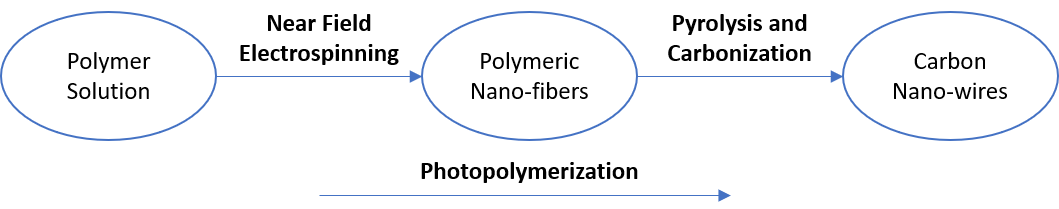
\includegraphics[width=0.95\textwidth]{./Figures/FabricationProcess.png}
%\decoRule
%\caption[Carbon Nano-wires Fabrication Process]{Fabrication process of carbon nano-wires to achieve through the proposed dissertation.}
%\label{fig:fabricationFlowChart}
%\end{figure}

%\begin{equation}
%\left(\tau _t^e-\frac{\tau _n^e \text{dr}}{\text{dz}}\right) 2 \pi  r+\frac{d \left(\pi  r^2
%   \left(\tau _{\text{zz}}-p\right)\right)}{\text{dz}}+\frac{\gamma  \text{dr} 2 \pi  r}{r
%   \text{dz}}+\rho  g \pi  r^2=\frac{d \left(\rho  \pi  r^2 v^2\right)}{\text{dz}}
%\label{eq:linearMomentum}
%\end{equation}
%% Chapter Template

\chapter{Problem Definition and Motivation} % Main chapter title

\label{Chapter:ProblemDefinitionandMotivation}

%\subsubsection*{\color{mygray}[Chapter ready for review]}
% Describe the current situation of this problem.
% identifying the obstacles and the possible applications of your research.
% background of the problem (e.g. origins, previous attempts, etc.). 
% State the problem in detail mentioning all relative aspects, variables, relationships,
% stressing on the importance of finding a solution to the problem.

Carbon nanowires have been fabricated with a photoresist by multiple-photon polymerization techniques. However little is known about polymers that can produce conductive carbon nano-wires after pyrolysis. The lack of research relays on the fact that in the past years, it was assumed that most polymers are non-graphitic through pyrolysis \cite{Franklin1951}. In the past years photon polymerization processes have been applied to the fabrication of nano-structures with the use of a epoxy based photoresist. \cite{Boer2014} Photon polymerization techniques deliver patterning resolutions with nano-scale tolerances for the production of highly detailed structures \cite{Hribar2014}.

On the other hand, electrospinning has been acknowledged as a process with promising results at nano-structure fabrication \cite{Boer2014}, yet there is little research regarding the implementation of electrospinning for the fabrication of carbon nano-wires. Electrospinning has the potential to be a more straightforward process for the design and fabrication of nano-structures, as it can achieve mass scale manufacturing in a continuous, simple and reproducible manner. Cárdenas \cite{Cardenas2017} shows that electrospinning can be implemented with ease for carbon nano-wire synthesis. Mechano-electrospinning, a new variant of electrospinning shows promising results in the production of ordered carbon nano-wires. As stated in \cite{Cardenas2017}, mechano-electrospinning is an early technology invention, and brings new challenges, such as the reproducibility of carbon nano-wire production. Furthermore, the study of a new fabrication process to produce carbon nanowires that involves mechano-electrospinning will enable spatial control of the structures' patterning.

Since electrospinning seems to be a better alternative for carbon nano-wire fabrication processes; and for that purpose of its implementation, it is required to develop polymer solutions that can be mechano-electrospun, photopolymerized and pyrolyzed into conducting carbon nano-wires. Carbon nano-materials have been subjected to research due to their various potential applications in diverse areas that take advantage of the nano-scale properties. \cite{Siddiqui2019} Carbon nano-materials are suitable for the catalysis, adsorption, carbon capture, energy and hydrogen storage, drug delivery, bio-sensing and cancer detection. \cite{Siddiqui2019} However most applications are not currently feasible due to the lack of a continuous, simple and reproducible fabrication method with inexpensive processes. With the newly designed polymer solution, it would be possible to produce carbon nano-wires in large quantities, and therefore more applications will become feasible. On the other hand, the new technique will overcome some limitations of other methods such as lithography currently has. For instance, patterns created by lithography processes cannot be originated, only replicated, all cinstituent points of the pattern can only be addressed at the same time, and the process requires the pattern to be encoded into a mask. \cite{Landis2011}  


%----------------------------------------------------------------------------------------
%	SECTION 1
%----------------------------------------------------------------------------------------



%-----------------------------------
%	SUBSECTION 1
%-----------------------------------


%% Chapter Template

\chapter{Hypothesis and Research Questions} % Main chapter title

\label{Chapter:HypothesisandResearchQuestions}

%\subsubsection*{\color{mygray}[Chapter ready for review]}
% The system/technique/parameter X is better, for task Y, than each of its rivals Z, in dimension W.

\section{Research Hypothesis}

The rheological properties of polymer solutions along with synthesis parameters (stage velocity, voltage, dispense rate) can be amended through rheological analyses to obtain a low voltage electrospun-able, photopolymerizable and graphitizable fibers for the synthesis of carbon nano-wires with specified dimensions (diameter and length). The rheological properties of polymer solutions along with synthesis parameters are to be amended by replacing the PEO (Poly(ethylene) oxide) component within the existing polymer solutions described in Flores \cite{Flores2017} and Cardemas \cite{Cardenas2017} work. PEO is to be replaced as its only purpose is to allow the electrospinning process to take place, but not benefit is obtained from it after pyrolysis.

\section{Research Questions}

\begin{itemize}
	\item{
	Is there any evidence of carbon nano-wire fabrication though electrospun-able and pyrozable polymer solutions?
	}
	\item{
	What are the process parameters to consider/control for the fabrication processes of carbon nano-wires? 
	}
	\item{
	What rheological properties are to be controlled/tested to deliver a electrospun-able and pyrozable polymer solution?	
	}
	\item{
	Are there any efforts employed to the design of polymer solutions that can be electrospun, photopolymerized, and pyrolyzed into conducting carbon nanowires?
	}
	\item{
	Are the optimal fabrication parameters defined \cite{Cardenas2017} for the synthesis of carbon nano-wires through near-field electromechanical spinning?	
	}
	\item{
	What PEO-similar materials can be used to allow the electrospinning technique and favor the carbon nano-wire properties after pyrolysis? 
	}
\end{itemize}

%----------------------------------------------------------------------------------------
%	SECTION 1
%----------------------------------------------------------------------------------------



%-----------------------------------
%	SUBSECTION 1
%-----------------------------------


%% Chapter Template

\chapter{Objectives} % Main chapter title

\label{Chapter:Objectives}

%\subsubsection*{\color{mygray}[Chapter ready for review]}
% Here you are meant to stipulate, in a broadly and specific way, what you want to achieve regarding the target problem. You may include the scope of your proposed research or any other element that you consider might set the boundaries of your work.
% This section can also present the Solution Model which is the one you propose to solve the problem. Obviously, this model has to be consistent with the objectives that have already set up. This model is the one that guides the research work and that, eventually, leads to the PERSONAL CONTRIBUTION.

\section{General objective}
Study the practice and feasibility of a new synthesis process to achieve mass scale manufacturing of carbon nano-wires in an inexpensive, continuous, simple and reproducible manner; by the integration of mechano-electrospinning technique.

\section{Particular objectives}

\begin{itemize}
	\item{
	Design polymer solutions that can be electrospun by NFES, photopolymerized, and then pyrolyzed.
    }
    \item{
    Through rheological analyses, determine if polymer solutions can be easily employed for conducting carbon nano-wire synthesis.
    }
    \item{
    Determine and control the polymer solution rheological properties along with the process parameters of carbon nano-wire synthesis.
    }
    \item{
    Discover a PEO-similar material to allow the electrospinning process as well as input favourable properties to the carbon nano-wire yield.
    }
\end{itemize}

%----------------------------------------------------------------------------------------
%	SECTION 1
%----------------------------------------------------------------------------------------



%-----------------------------------
%	SUBSECTION 1
%-----------------------------------
%% Chapter Template

\chapter{Related Work} % Main chapter title

\label{Chapter:RelatedWork}

%\subsubsection*{\color{mygray}[Chapter under work]}

%----------------------------------------------------------------------------------------
%	SECTION 1
%----------------------------------------------------------------------------------------

\section{Role of rheological properties in near field electrospun fibers morphology \cite{Flores2017}}

Flores studied SU-8 2002 polymer solutions in cyclopentanone with poly(ethylene) oxide (PEO) and tetrabutylammonium tetrafluoroborate (TBATFB). For that purpose, several samples were prepared with the adequate amounts of PEO and TBATFB with 5 $m l$ of SU-8 2002 and stirred at 160 $r p m$ for one hour at 75 $^\circ C$ in the absence of light. A 5 $m l$ syringe was used to extract the solution from the preparation vial. Finally the syringe was placed upside down for 24 hours to get rid of any bubbles within the solution. Table \ref{tbl:FloresSamples} lists the set of samples that were prepared as values in $w t \%$, dissolved in SU-8 2002.

\begin{table}[th]
\caption{Set of prepared samples}
\begin{center}
\begin{tabular}{ c c c c c c c } 
\hline
\text{} & \multicolumn{2}{c}{Serie A} & \multicolumn{2}{c}{Serie B} & \multicolumn{2}{c}{Serie C} \\
\hline
Sample & PEO & TBATFB & PEO & TBATFB & PEO & TBATFB \\
\hline
1 & 0.00 & 0.00 & 0.00 & 0.50 & 0.50 & 0.00 \\
2 & 0.25 & 0.25 & 0.25 & 0.50 & 0.50 & 0.25 \\
3 & 0.50 & 0.50 & 0.50 & 0.50 & 0.50 & 0.50 \\
4 & 0.75 & 0.75 & 0.75 & 0.50 & 0.50 & 0.75 \\
5 & 1.00 & 1.00 & 1.00 & 0.50 & 0.50 & 1.00 \\
\hline
\label{tbl:FloresSamples}
\end{tabular}
\end{center}
\end{table}

All the samples were executed in a rheometer (Physica MCR 301, Anton Paar) with a cone-and-plane geometry of diameter 24.979 $m m$, angle 4.014$^\circ$ and truncation of 249 $\mu m$. The measurements were performed at a temperature of 25 $\pm$ 0.1 $^\circ C$. For amplitude sweep measurements, the angular frequency was settled at 10 $s^{-1}$, and the percentage amplitude gamma $\% \gamma$, was varied from 0.1 to 1000\%. In flow curve tests, shear rate was applied from 0.1 to 100 $s^{-1}$. For frequency sweeps, the percentage of amplitude gamma, $\% \gamma$, was varied from 0.1 to 100 $s^{-1}$. During the measurements, the rheometer sample area was saturated with cyclopentanone to avoid solvent evaporation.

\subsection{Rheological Characterization : \textbf{Amplitude Sweep}}
The "Serie A`` result measurements indicate that the storage modulus $G'$ is smaller than the loss modulus $G''$. Both moduli have a parabolic behaviour. At low deformation the values of the moduli increase until they become stable at between 1 and 10 $\% \gamma$. After the stabilization, both modulus start to decrease. The increase of PEO and TBATFB concentration $G'$ and $G''$ also increase. Figure \ref{fig:SerieAampSweep} shows the amplitude sweep for the samples of "Serie A``.

\begin{figure}[th]
\centering
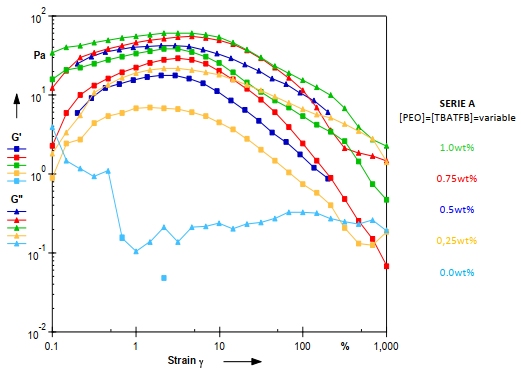
\includegraphics[width=0.75\textwidth]{./Figures/SerieAampSweep.png}
\decoRule
\caption[Serie A - Amplitude Sweep]{Serie A - Amplitude Sweep}
\label{fig:SerieAampSweep}
\end{figure}

The results within Figure \ref{fig:SerieAampSweep} showed that no clear linear viscoelastic region is present. The material has influenced by small deformations, hence it is very sensible to external forces. No yield point was encountered as the moduli separate from each other with the increase of deformation.

Figure \ref{fig:SerieBampSweep} illustrates the results obtained from the amplitude sweeps of Serie B samples. As shown in the figure, the concentration of 0 $w t \%$ shows a constant viscous modulus at 0.2 $Pa$. the 0.25 $w t \%$ concentration sample presented a similar behaviour to the 0 $w t \%$ sample but with a constant value of $G'$ at 2 $Pa$. The other concentrations show a similar parabolic behaviour as the ones in Serie A.

\begin{figure}[th]
\centering
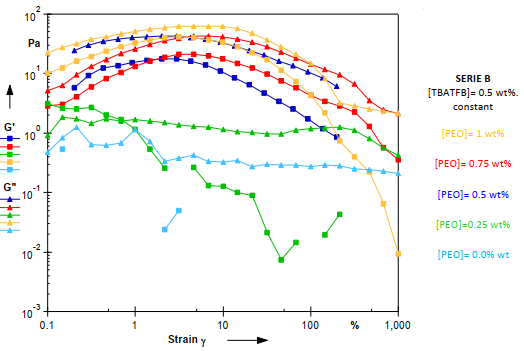
\includegraphics[width=0.75\textwidth]{./Figures/SerieBampSweep.png}
\decoRule
\caption[Serie B - Amplitude Sweep]{Serie B - Amplitude Sweep}
\label{fig:SerieBampSweep}
\end{figure}

\begin{figure}[th]
\centering
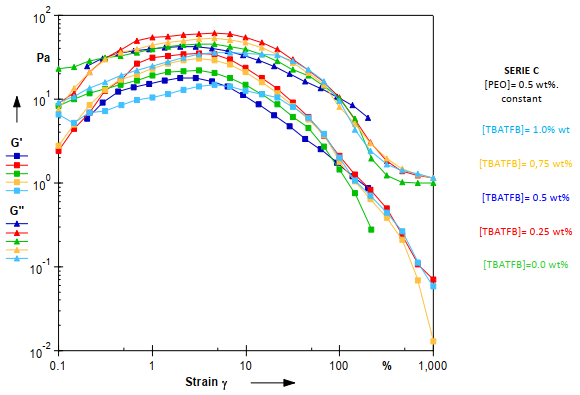
\includegraphics[width=0.75\textwidth]{./Figures/SerieCampSweep.png}
\decoRule
\caption[Serie C - Amplitude Sweep]{Serie C - Amplitude Sweep}
\label{fig:SerieCampSweep}
\end{figure}

The amplitude sweep results of Serie C are depicted in Figure \ref{fig:SerieCampSweep}. Similar to series A and B, results show that the storage modulus $G'$ is smaller than the loss modulus $G''$ with a parabolic behaviour. Typically, the amplitude sweep is to determine the amplitude to be used in frequency sweeps. The amplitude determined by the amplitude sweeps shall keep the material structure undisturbed is known as the linear viscoelastic region (LVER). However, no LVER was found in the samples. For that reason, the percentage of amplitude gamma $\% \gamma$ was found by trial and error. Flores discovered that a $\% \gamma = 20$ has the best performance. 

\subsection{Rheological Characterization : \textbf{Flow Curve}}
Figure \ref{fig:SerieAflowCurve} shows evidence that the equal increase of PEO and TBATFB concentrations result in an increase of shear viscosity rate $\gamma$. for concentrations from 1.00 to 0.25 $w t \%$, a slight increase of flow curve strain $\eta$ for low shear rates to 0.3 $s^{-1}$. For shear rates greater than 0.3 $s^{-1}$, the $\eta$ starts to decrease, as the polymer entanglements start to break apart, reducing friction between the polymer threads and therefore the viscosity also is reduced. The solution samples show a Newtonian-like behaviour and that may be caused by the use of the solvent cyclopentanone and by the small sized SU-8 2002 molecules.

\begin{figure}[th]
\centering
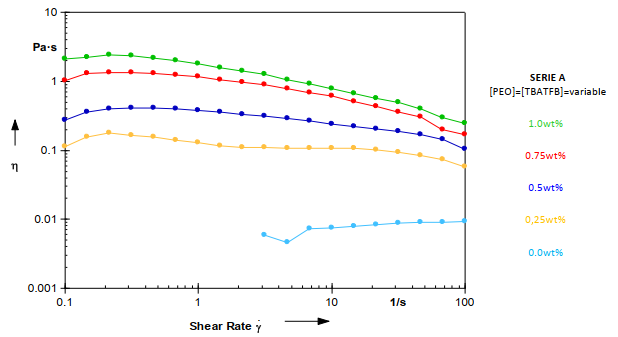
\includegraphics[width=0.75\textwidth]{./Figures/SerieAflowCurve.png}
\decoRule
\caption[Serie A - Flow curve]{Serie A - Flow curve}
\label{fig:SerieAflowCurve}
\end{figure}

From the results in Figure \ref{fig:SerieAflowCurve}, it is noticeable that the addition of small amounts of PEO and TBATFB cause a change of one order of magnitude in shear viscosity in small concentration and a triple change in high concentrations.

Series B flow curve results (Figure \ref{fig:SerieBflowCurve}) do not show a clear correlation between PEO concentrations and shear viscosity. For PEO of 1 $w t \%$, a slow increase in $\eta$ is present with the increase of shear rate, after $\gamma$ drops from 2 to 0.8 $Pa s$, a shear thinning behaviour is present. For 0.50 and 0.75 $w t \%$ concentrations, a shear thinning behaviour is present throughout the plot. For the 0.50 $w t \%$ sample, viscosity value varied between 0.2 and 0.4 $Pa s$; and between 0.5 and 2.0 $Pa s$ for the 0.75 $w t \%$ sample. Viscosity is stabilized at 0.1 $Pa s$ when the shear rate is between 1 and 20 \% for the sample of PEO $w t \%$. After stabilization, the viscosity decreases from 0.1 to 0.02 $Pa s$ for shear rates between 20 to 100 $s^{-1}$. For PEO 0.00 $w t \%$, a high variation is present in viscosity readings due to the presence of electrolytes cause amendments in the polymer chain within the solution.

\begin{figure}[th]
\centering
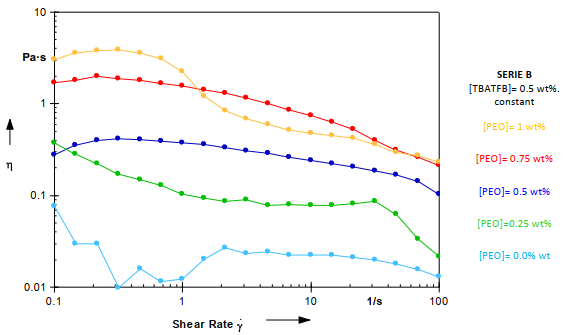
\includegraphics[width=0.75\textwidth]{./Figures/SerieBflowCurve.png}
\decoRule
\caption[Serie B - Flow curve]{Serie B - Flow curve}
\label{fig:SerieBflowCurve}
\end{figure}

The flow curve results of Serie C are presented in Figure \ref{fig:SerieCflowCurve}. The sample with 1 $w t \%$ TBATFB concentration shows a shear thinning behaviour for shear rates varying between 0.1 to 15 $s^{-1}$. The 1 $w t \%$ sample describes a drop in viscosity for shear rates between 15 to 20 $s^{-1}$ followed by a stable state. A similar behaviour is observed for concentration of 0.75 $w t \%$. and less evident for 0.0 $w t \%$. For concentrations of 0.5 $w t \%$ and 0.25 $w t \%$ the behaviour of the shear viscosity is similar.

\begin{figure}[th]
\centering
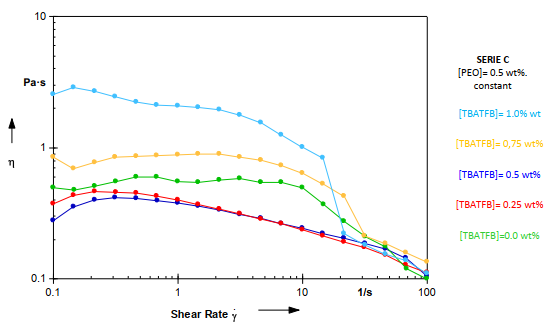
\includegraphics[width=0.75\textwidth]{./Figures/SerieCflowCurve.png}
\decoRule
\caption[Serie C - Flow curve]{Serie C - Flow curve}
\label{fig:SerieCflowCurve}
\end{figure}

\subsection{Rheological Characterization : \textbf{Frequency Sweep}}
Figure \ref{fig:SerieAfreqSweep} shows that the solution with the lowest concentration of PEO and TBATFB has a decreasing behaviour of the viscosity, but for values greater to 3 $s^{-1}$ in frequency, the viscosity starts to increase. The solutions from 0.25 $w t \%$ to 1.00 $w t \%$ have the same shear-thinning behaviour. A direct relation between the concentrations and the viscosity values is discovered, where a small drop of viscosity is presented with the decrease of additive concentration.

\begin{figure}[th]
\centering
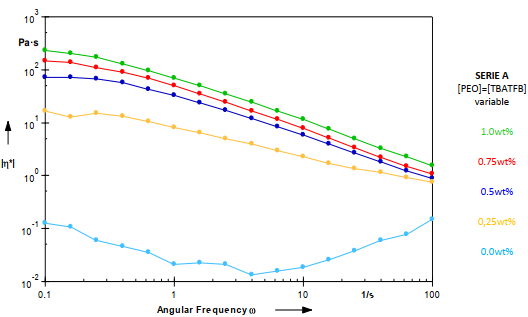
\includegraphics[width=0.75\textwidth]{./Figures/SerieAfreqSweep.png}
\decoRule
\caption[Serie A - Frequency Sweep]{Serie A - Frequency Sweep}
\label{fig:SerieAfreqSweep}
\end{figure}

Figure \ref{fig:SerieBfreqSweep} shows the frequency sweep results from Serie B. The presented behaviour is similar to Serie A. for the lower concentrations of PEO, the equipment has not enough sensibility to make measurements of the storage modulus because this one is very low. At PEO 0.25 $w t \%$, the viscosity remains almost constant at 1 $Pa s$, but as in Serie A a little variation of viscosity is presented at the lowest values of angular frequency. On the other hand, for the 0.5, 0.75 and 1.00 $w t \%$ concentrations, the viscosity is similar. At 100 $s^{-1}$, the three high concentration samples converge to 2 $Pa s$. It is imperative to assume that 0.5 $w t \%$ is the critical concentration, under this concentration the systems presents different behaviours since the molecules have enough room to diffuse and break entanglements. When the critical entanglement concentration is exceeded, the polymer threads overlap and become tangled, therefore no more entanglements are no longer possible.

\begin{figure}[th]
\centering
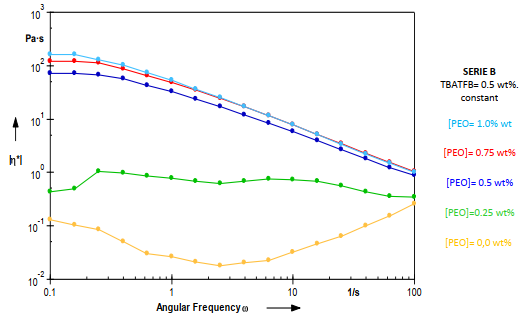
\includegraphics[width=0.75\textwidth]{./Figures/SerieBfreqSweep.png}
\decoRule
\caption[Serie B - Frequency Sweep]{Serie B - Frequency Sweep}
\label{fig:SerieBfreqSweep}
\end{figure}

The frequency sweep behaviours of Serie C are presented in Figure \ref{fig:SerieCfreqSweep}. The figure does not indicate a clear correlation between the viscosity and the addition of TBATFB. All samples have a similar behaviour and magnitude, except for the 0.75 $w t \%$ TBATFB concentration sample as it presents a non uniform behaviour. At low frequencies, the viscosity increases, then it remains constant at 20 $Pa s$ until a frequency value of 4 $s^{-1}$; the viscosity drastically decreases to 1 $Pa s$ and remains constant at that value. The 1.00 $w t \%$ sample has a decreasing viscosity behaviour at higher angular frequencies. 

\begin{figure}[th]
\centering
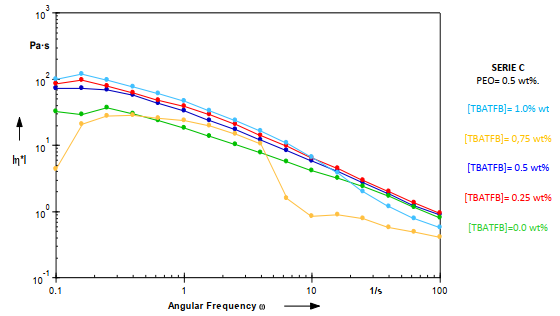
\includegraphics[width=0.75\textwidth]{./Figures/SerieCfreqSweep.png}
\decoRule
\caption[Serie C - Frequency Sweep]{Serie C - Frequency Sweep}
\label{fig:SerieCfreqSweep}
\end{figure}

Flores work \cite{Flores2017} carried out a series of experiments in order to correlate the rheological properties of polymer solutions used in electro-mechanical spinning processes for the fabrication of carbon micro structures. Shear flow and dynamic measurements tests such as flow curves, amplitude sweeps and frequency sweeps were carried in an oscillatory rheometer to study the rheological behaviour of polymeric solutions of SU-8 2002, an epoxy-based negative photoresist, Poly(ethylene) oxide (PEO), a flexible, non-ionic polymer, and TBATFB (Tetrabutylammonium tetrafluoroborate) that acts as an electrolyte.

The concentrations of additives were varied from 0 $w t \%$ to 1.0 $w t \%$ with increments of 0.25. To observe the effects of each additive it was proposed a set of concentrations where both additives were equally varied (Serie A), TBATFB was constant the only PEO variations (Serie B), and PEO constant concentration with TBATFB variations (Serie C). It was found that the variation of the additives (PEO and TBATFB) affects the
rheological behavior of the solution. Typically, the addition of PEO increase the
elongational and shear viscosities while the addition of TBATFB modifies this property
but in a non-predictable manner. The solutions do not present yield stress as can be
seen in Amplitude Sweep and Frequency Sweep measurements.

\clearpage

\section{Advanced Manufacturing Techniques for the Fabrication and Surface Modification of Carbon Nanowires \cite{Cardenas2017}}

As stated by Cardenas \cite{Cardenas2017}, the following parameters play an important role in the graphitic content on the fabrication of carbon nano-wires through electrospinning:

\begin{enumerate}
\item The thickness of the produced polymeric wires,
\item the chemical composition and viscoelasticity of the polymeric solution,
\item the molecular alignment of the polymer,
\item the heat treatment temperature,
\item the mechanical pulling on the polymer jet during electrospinning,
\item the alifnment of polymer chains induced by the presence of an electric field, and
\item the catalysts and solvents within the polymer solution.
\end{enumerate}

Cardenas reviewed different polymer fabrication techniques and materials to produce carbon nano-wires. Within Cardenas' work the following parameters were evaluated to study the desirable characteristics for building highly sensitive sensor devices: a) the chemical composition and viscoelasticity of the polymer solution, b) the thickness of the produced polymeric wires, c) the mechanical pulling on the polymeric jet during electrospinning, and d) the alignment of the polymer chains induced by the presence of an electric field. Cardenas' work states that various methods are implemented to produce nanofibers, such as laser ablation, chemical vapor deposition, discharge, and vapour growth. However, those techniques are abandoned due to their low yield output and expensive equipment. Whereas electrospinning (ES) of polymer solutions is a promising technique for simple and inexpensive fabrication of carbon nano-wires, which can be combined with a moving collector to yield even thinner fibers.

The production of carbon sstructures involves to main procedures: a) polymer patterning such as photolithography, electrospinning, Computer Numerical Control (CNC), moulding, hot embossing, and recently, Multiple Photon Polymerization; and b) carbonization, which induces further thinning of the patterned polymer and its conversion into carbon. Cardenas conducted some experiments to characterize and analyse carbon nano-wires. Polymeric SU-8 nano fibers were produced by two different methods; for each method different polymer solutions were employed.

\subsection{Method 1 : }

\subsubsection{Polymer Solution}
The polymeric solution was composed by 2 $ml$ of SU-8 2002 mixed with 0.5 $w t \%$ of PEO and 0.5 $w t \%$ of TBATFB to increase its conductivity and yield soother polymer jets during electrospinning. Magnetic stirring was performed for 1 $hr$ at 75 \textdegree{}$C$ with $rpm$ values between 100 and 150.

\subsubsection{Deposition}
A voltage around 100 $V$ was applied between a dispensing needle and the collector stage. The needle to collector distance was set to 100 $\mu m$. The collector was attached to a mechanically motorized stage, which allowed the SU-8 nanofibers patterning into the SU-8 microstructures. Three different stage velocities were tested (20,40 and 60 $mm/s$) to study the influence on the wire geometry. Acceleration of the stage was set to 500 $mm/s^{2}$. After deposition, samples were exposed to UV light for 45 $min$ to complete cross-linking.

\subsection{Method 2 : }

\subsubsection{Polymer Solution}
The solution was composed of 4 $ml$ of SU-8 2025, 4 $mg$ of TBATFB and 80 $\mu L$ of SU-8 thinner. The solution was stirred for 1.5 $hrs$ at 100 $rpm$ at 75 \textdegree{}$C$.

\subsubsection{Deposition}
To pattern the fiber exactly on top of the SU-8 electrodes, a routine was set to move the needle relative to the collector. The polymer solution was dispensed at a rate of 8.847 $nL / min$ using a programmable syringe pump. A voltage of 200 $V$ was applied between the collector plate and the needle tip, and the polymer solution was allowed to flow for between 15 to 30 $min$ until it was stable. A higher voltage had to be applied compared to Method 1 due to the higher viscosity of the SU-8 2025 solution. Once a steady flow was achieved, the collector was moved relative to the needle tip using the motorized stage. The mechanical parameters used during were: a) velocity of 5000 $\mu m/s$, an acceleration of 2500 $\mu m/s^{2}$. The sample was exposed to UV light for 45 min to ensure complete cross-linking of the deposited SU-8 nanofiber.

\subsection{Results and Discussion}
To test the possibility of using SU-8 to fabricate carbon nano-wires, samples were pyrolyzed in an inert environment. Samples prepared by Method 1 failed the pyrolyzation as the deposited wires were mostly liquid before carbonization. The fibers produced by Method 2 had a yeild rate of 81 $\%$. The diameters after pyrolysis were analyzed and measured using SEM micrographs.

Cardenas \cite{Cardenas2017} states that the geometry of the carbon nano-wires is also an important characteristic that affects the carbon structure conductivity, mechanical and thermal characteristics and crystallinity. The conducted experiments showed some techniques and materials that have been applied to fabricate carbon nano-wires, as well as the effects that fabrication parameters have on the final geometry of the carbon structures. The newly technique of electro-mechano-spinning (EMS) involved new polymer solutions along with a systematic deposition process. Cardenas found that the EMS proposed manufacturing technique yielded normally distributed diameters of 204 $nm$ with low variability, which is significantly reduced the uncertainty in the fabrication of carbon nano-wires.

\section{Effect of pyrolysis process parameters on electrical, physical, chemical and electro-chemical properties of SU-8-derived carbon structures fabricated using the C-MEMS process \cite{Pramanick2018}}


%-----------------------------------
%	SUBSECTION 1
%-----------------------------------



%% Chapter Template

\chapter{Theoretical Framework} % Main chapter title

\label{Chapter:TheoreticalFramework}

%\subsubsection*{\color{mygray}[Chapter under work]}
% Background and state-of-the-art
% This involves a thorough state-ofthe-art bibliographic review, the building of a formal foundation, the study of related techniques, analysis and awareness of previous works and study of fundamental aspects that can help carry on your research.

\section{Photoresists}
The electronic industry requires sustainable raw material supply for its development \cite{Sutikno2016}. Photoresists are a type of raw material used in microelectronics, which is composed by four main elements: a polymer (resin), a photoactive compound, a solvent, and an additive \cite{Schuster2009}. The additive requires to be with a low molecular weight as it is intended to act as a photosensitive material. Photoresists are used within the manufacturing process of printed circuit boards \cite{Staab2011}. Photoresists are classified into two categories. The resist is defined as positive if the radiation exposed material is soluble in photoresist developer; otherwise, for negative photoresist the exposed material remains to stay in the photoresist surface as it crosslinks upon exposure \cite{Landis2011,Sharma2012}. In the manufacturing process of a semiconductor, the radiation sources which are often used in a lithography process are ultraviolet (UV) and X-ray \cite{Mekaru2015}.

The polymeric material is available on the broad market either in liguid or solid state; \emph{MicroChem Corp.} (Westborough, MA, USA) is the principal provider of SU-8 photoresist. SU-8 and similar photoresists are inexpensive with good adhesion on the semiconductor surface and high sensitivity \cite{Staab2011}. Epoxy resins are copolymer-thermosetting plastics which are normally produced by a chemical reaction process that involves epichlorohydrin and bisphenol-A compound \cite{Singla2010}. A epoxy-based polymer is typically used to produce patterns by lithography with the application of UV radiation. Lithography is a technique to transfer patterns from a mask and then transferred onto the substrate \cite{Landis2011,Xu2014}. SU-8 is a epoxy-based negative photoresist with the advantages of being inexpensive with good mechanical properties, good chemical resistance, and good electrical isolation \cite{Xu2014}. SU-8 photoresists are used in the production processes of MEMS \cite{Zhang2001}. Photoresist-wise, the contrast and quality level of UV radiation lithography is affected by the wavelengths of radiation sources. The higher the sensitivity of the material, the better is the lithography process as it absorbs radiation energy with ease to perform photochemical reactions in forming patterns \cite{Zhang2001}.

In summary, a photoresist is a "epoxy-based resin (polymeric) material which changes its dissolution rate in a liquid solvent, called a developer, under high energy radiation.`` \cite{Landis2011}

\section{Electro-Mechanical Spinning}
Diverse polymer patterning techniques have being develop for the fabrication of nano-fibers, such as arc discharge \cite{Wang2007}, chemical vapor deposition, laser ablation \cite{Ren1998}, and vapor growth \cite{Nadarajah2008}. Nonetheless, those processes are expensive due to either the low product yield or the expensive equipment required. The electrospinning method (invented by Formhals Anton in 1934) can produce fibers with a range of diameters between 10 $n m$ and 10 $\mu m$ \cite{Jayaraman2003,Anton1930} from a polymer solution under the influence of an electrostatic force. The applied electric field and solution conductivity and viscosity is an important parameter the affects the fiber diameter during the spinning along with other parameters such as jet length, solution viscosity surrounding gas, flow rate and the collector geometry \cite{Anton1938,Larrondo1981,Baumgarten1971,Shin2001}.

Even though electrospinning is an old invention \cite{Anton1930}, it is currently a trending topic among researchers \cite{Huang2003,Reneker2008,Schiffman2008}. Some of the reasons electrospinning is to be studied is its potential to fabricate polymer nano-fibers from a variety of polymers. The technique allows the production of thin continuous fibers with ease, with diameters down to 3 $n m$ in some cases, which is something difficult to achieve by other techniques. Furthermore, the basic set-up can be modified with ease to fabricate different fibers with diversified functionalities with different materials. The produced fibers can be aligned or unaligned. Besides, the electrospinning equipment is inexpensive and of small size, compared to the equipment of standard spinning techniques. On the other hand, the understanding of the electrospinning process has improved in the last years \cite{Li2012}. As Reneker and Yarin state: "Electrospinning has rapidly changed fiber making from a capital intensive, large scale process to a low cost, broadly applicable method that manufactures fibers on a laboratory bench, to serve diverse needs ranging from materials science and technology to life sciences and clinical medicine.`` \cite{Reneker2008}

The main components of the electrospinning technique are the fluid control unit (e.g. syringe pump) and a DC power supply. The process also requires a target electrode or combination of electrodes on which the fibers can be collected. Figure \ref{fig:FFES} describes a typical electrospinning set-up. \cite{Li2012}

\begin{figure}[th]
\centering
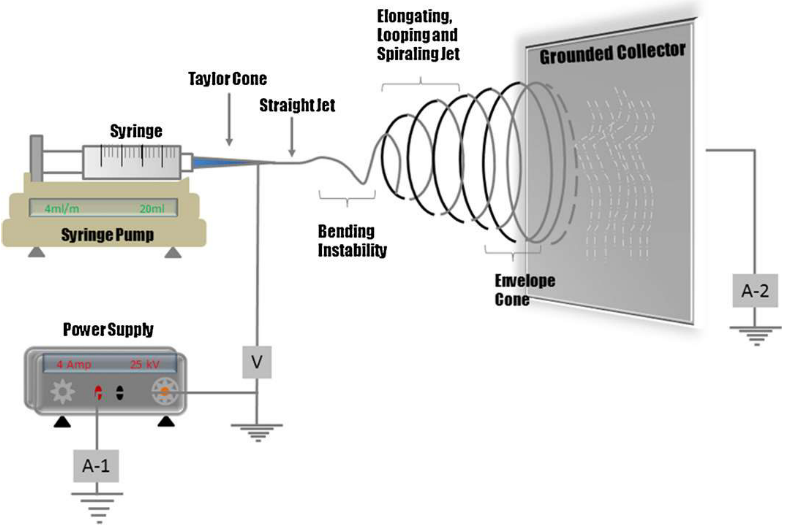
\includegraphics[width=0.75\textwidth]{./Figures/FFES.png}
\decoRule
\caption[Far Field Electrospinning set-up]{Typical far field electrospinning (FFES) set-up \cite{Li2012}.}
\label{fig:FFES}
\end{figure}

Two sub-techniques can be derived from electrospinning depending on the distance between the dispensing electrode and the collector. The process in which the electrospun jet can be controlled near the tip is called NFES or near-field electrospinning. \cite{Cisquella-Serra2019} Moreover, if the distance between the collector and the dispensing needle is farther, the configuration is known as FFES or far-field electrospinning. \cite{Nataraj2012} The difference between NFES and mechano-electrospinning is the presence of a mechanical collector that allows higher precision when patterning. Figure \ref{fig:NFES} shows a typical near field mechano-electospinning apparatus.

\begin{figure}[th]
\centering
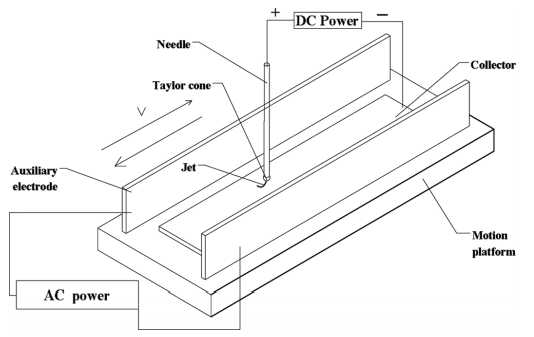
\includegraphics[width=0.75\textwidth]{./Figures/NFES.png}
\decoRule
\caption[Near Field Electrospinning set-up]{Typical near field electrospinning (NFES) set-up \cite{Zhu2016}.}
\label{fig:NFES}
\end{figure}

\section{Pyrolysis}
Pyrolysis is technique that involves heating of biomass in the absence of air or oxygen at a maximum pyrolysis temperature. A small amount of oxygen can burn the structures and make them unusable \cite{Pramanick2018}. Once the maximum pyrolysis temperature is reached, the temperature remains constant to produce solid char, liquids, and non-condensable products. In most cases the liquid product is the main interest of the pyrolysis process, and the properties of the pyrolysis products depend on the maximum pyrolysis temperature and the heating rate \cite{Pramanick2018,Basu2018}.

The heating of large biomass molecules results in decomposition. The pyrolysis decomposition process comprises char, liquids (condensable gases) and non-condensable gases; where the consensable gases may suffer further decomposition into non-condensable gases such as $C O$, $C O_{2}$, $H_{2}$, and $C H_{4}$. Equation \ref{eq:genPyrolysis} is a general representation of the pyrolysis decomposition reaction \cite{Basu2018}.

\begin{equation}
C_{n} H_{m} O_{p} (biomass) \overset{heat}{\rightarrow} \underset{liquid}{\Sigma} C_{x} H_{y} O_{z} + \underset{gas}{\Sigma} C_{a} H_{b} O_{c} + H_{2} O + C (char)
\label{eq:genPyrolysis}
\end{equation}

Pyrolysis yields solid products that are more energy dense than the initial biomass, however the gas and liquid products are less energy dense \cite{Basu2018}. The liquid product of pyrolysis is usually of colour black containing hydrocarbons with a large amount of oxygen and 20\% water. When the liguid product is of interest, a rapid "quenching`` (freeze) is required after pyrolysis to prevent further decomposition or reaction with other substances \cite{Basu2018}. The solid yields of pyrolysis is usually around 85\% carbon with some oxygen, hydrogen and other substances that are present within the initial biomass \cite{Basu2018}. The biomass decomposition by pyrolysis produces non-condensable and condensable gases. The vapors (condensable gases) add up to the liquid yield of pyrolysis which is generated upon cooling. The gases (non-condensable gases) are comprised by ethylene, ethane, methane, carbon monoxide and carbon dioxide \cite{Basu2018}.

\section{Carbon nano-wire}
Carbon nano-wires (CMWs) are known as long, thin strings with diameters between 10 and 1 thousand $n m$; composed mostly by carbon atoms aligned parallel to the long axis of the fiber \cite{Nataraj2012}. Carbon nano-wires are different from carbon nano-tubes, as CMWs are not composed by graphene sheets in cylindrical form \cite{Nataraj2012}. Carbon nano-wires are typically fabricated by electrospinning and pyrolysis/carbonization as the main processes. During the fabrication process, the polymer molecules are to be crosslinked to prevent melting during the subsequent pyrolysis. The carbonization step removes non-carbonized components in form of condensable and incondensable gases \cite{Basu2018} to then yield carbon structures of about 50\% to 75\% of the mass of the original polymeric structure \cite{Nataraj2012}.

\section{Polymer Solutions}
Polymer solutions display viscoelastic properties that provide unique properties due to their macromolecules. their chains are long and entangled. When a shear force is applied, the solution creates a large interaction between the molecules, hence the viscosity depends not only on temperature and shear, but also molecular weight distribution and concentration. The solvent also affects the viscosity \cite{Flores2017, Huang2003, Baumgarten1971}.

\begin{figure}[th]
\centering
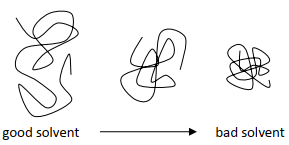
\includegraphics[width=0.50\textwidth]{./Figures/goodbadsolvent.png}
\decoRule
\caption[Effects in polymer chains dimensions due to solvent quality]{Effects in polymer chains dimensions due to solvent quality \cite{Flores2017}}
\label{fig:goodbadsolvent}
\end{figure}

Figure \ref{fig:goodbadsolvent} shows how the quality of a solvent affects the polymer distribution within the solution. Moreover the prsence of electrolites also modify the structure of the polymer threads. In non-ionic solvents, the charges are distributed along the chains and their own repulsion stretches the polimer threads into a more aligned configuration when an electrolyte is added, as detailed in Figure \ref{fig:electrolyteConcentration}.

\begin{figure}[th]
\centering
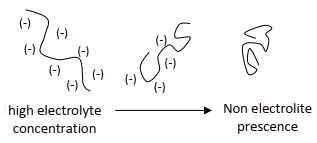
\includegraphics[width=0.50\textwidth]{./Figures/electrolyteConcentration.png}
\decoRule
\caption[Effects of electrolyte in polymer chain dimensions]{Effects of electrolyte in polymer chain dimensions \cite{Flores2017}}
\label{fig:electrolyteConcentration}
\end{figure}

\section{Rheometry}
Rheometry is the measuring technology used to determine rheological data. There are different measuring systems, instruments and analysis methods. Both, liquids and solid  can be investigated using rotational and oscillatory rheometers. Rotational tests are performed to characterize viscous behavior. In order to evaluate viscoelastic behavior, creep tests, relaxation tests and oscillatory tests are performed \cite{Flores2017}.

\subsection{Amplitude Sweep}
An amplitude sweep is a typical test used to characterize the behavior of a polymer
solution or polymer melt. In this basic test a constant angular frequency is applied along with an increasing or decreasing deformation or strain, see Figure \ref{fig:ampSweep} a). The obtained results are the storage and loss moduli, $G'$ and $G''$ respectively, along the values of percentage of strain applied. The amplitude is the maximum of the oscillatory motion. Normally at low frequencies the viscoelastic material presents a linear behavior, this is when the viscoelastic properties are independent of the strain or stress imposed due to the structure of the material stays undisturbed. Nevertheless, as the amplitude is increased at some at some point this linear trend changes suddenly. Once this critical amplitude value is reached the material becomes more elastic or viscous depending on the solution initial state, see Figure \ref{fig:ampSweep} b) \cite{Flores2017}.

\begin{figure}[th]
\centering
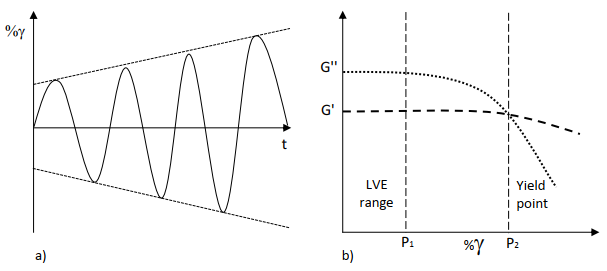
\includegraphics[width=0.75\textwidth]{./Figures/ampSweep.png}
\decoRule
\caption[Amplitude Sweep]{a) Imposed amplitude along time with constant frequency. b) Results for an amplitude sweep \cite{Flores2017}}
\label{fig:ampSweep}
\end{figure}

\subsection{Frequency Sweep}
A frequency sweep, is a common oscillatory test useful to understand the rheological behavior of fluids as it measures the viscoelastic properties. This measurement is considered a viscoelastic spectrum, in general, the shorter the timescale the more elastic the material behaves. These results are related to the molecular structure of the sample. Figure \ref{fig:freqSweep} shows a typical data for a polymer melt where different regions are observed. Frequency sweep measurements also allow the estimation of the molecular weight distribution characteristics such as entanglement density and process-ability \cite{Flores2017}. 

\begin{figure}[th]
\centering
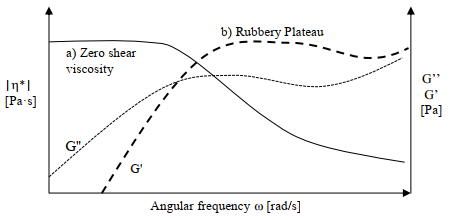
\includegraphics[width=0.75\textwidth]{./Figures/freqSweep.png}
\decoRule
\caption[Frequency Sweep]{Typical results for a frequency sweep. \cite{Flores2017}}
\label{fig:freqSweep}
\end{figure}

\subsection{Flow Curve}
The viscosity is measured as a function of the shear rate in a rotational rheometer with different geometries according to the sample. Normally three types of behaviours can be characterized in flow curve measurements: a) ideal viscous, b) shear thinning and c) shear thickening. Figure \ref{fig:flowCurve} shows three different materials and their response to an imposed shear rate \cite{Flores2017}.

\begin{figure}[th]
\centering
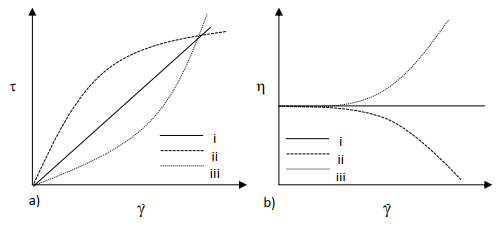
\includegraphics[width=0.75\textwidth]{./Figures/flowCurve.png}
\decoRule
\caption[Flow Curves]{a) Flow curve stress vs stress. b) Flow curve strain vs shear viscosity. Both figures for i Newtonian fluid, ii Shear thinning fluid, iii Shear thickening fluid. \cite{Flores2017}}
\label{fig:flowCurve}
\end{figure}

\section{Preliminary Experiments}


To verify Flores' work \cite{Flores2017}, a series of rheological measurements have been executed. Since one purpose of the proposed dissertation is to replace

%----------------------------------------------------------------------------------------
%	SECTION 1
%----------------------------------------------------------------------------------------



%-----------------------------------
%	SUBSECTION 1
%-----------------------------------



%% Chapter Template

\chapter{Methodology} % Main chapter title

\label{Chapter:Methodology}

%\subsubsection*{\color{mygray}[Chapter under work]}
% process or set of steps that are to take place in order to fulfill the objectives. These steps must mention the experiments to conduct, how they are going to be carried out, the evaluation of the obtained results, the validation of the hypothesis, the answers to the research questions, and the last step must be the written report of the outcomes

The following describes the proposed work to be done to fulfill the objectives stated in this document. The tasks are grouped in several work packages as described bellow:

%----------------------------------------------------------------------------------------
%	SECTION 1
%----------------------------------------------------------------------------------------

\section{Work package 1 : Preliminary Literature Review}
The first step to the thesis development is the study of preliminary literature and related work. The purpose of this work package is the familiarization of the existing techniques such as: far and near field electrospinning, lithography, pyrolysis, carbonization and photopolymerization. On the other hand, some research is to be done in order to recognize if there are any efforts in the design of electrospun-able, photopolymerizable and pyrolysable polymer solutions.

Furthermore, the motive of this work package is to find common parameters that could link the techniques mentioned above for the fabrication of carbon nano-wires from polymer solutions that can be electrospun by NFES, photopolymerized and then pyrolyzed. This work package is to be carried out through the entire thesis development process, as the state-of-the-art may change within that period of time.

\section{Work package 2 : Evaluation of Fabrication Parameters}
As the polymer solution is the principal input to the proposed technique (See Figure \ref{fig:fabricationFlowChart}), it is required to identify and understand the fabrication parameters that have an impact to the quality of the carbon nano-wires. For that reason two tasks are to be executed:

\begin{itemize}
	\item Study and identify the process parameters that influence the fabrication of carbon nano-wires
	\item Study and identify the rheological properties in polymer solutions that affect the electrospinning and pyrolysis techniques
\end{itemize}

\section{Work package 3 : Polymer Solution Design}
Once the process parameters and rheological properties that affect the fabrication of carbon nano-wires are identified, the design process shall take place. This work package is to study polymer solutions that can be electrospun by NFES, photopolymerized and pyrolyzed. The polymer solution design will comprise of two steps:

\begin{itemize}
	\item Prepare and test various polymer solutions with specific distinctions according to the identified solution properties and process parameters.
	\item Perform rheological analyses to determine if the prepared polymer solutions can be employed for the fabrication of carbon nano-wires.
\end{itemize}

\section{Work package 4 : Fabrication of Carbon Nano-wires}
From the rheological analyses, determine and control the polymer solution properties and fabricate carbon nano-wires.
	
This work package intends to involve several manufacturing processes (near field electrospinning, photopolymerization, pyrolization and carbonization) for the fabrication of carbon nano-wires. This task will require the integration of several techniques:

\begin{itemize}
	\item \emph{Electrospinning} - to convert the polymer solution into polymer nano-fibers
	\item \emph{Photopolymerization} - to change the chemical properties of the polymer solution and crosslink its molecules. This is to prevent the polymer to melt during pyrolysis \cite{Basu2018}.
	\item \emph{Pyrolysis} - to transform the polymer nano-fibers into conductive carbon nano-wires.
\end{itemize}

See Figure \ref{fig:fabricationFlowChart}.
	
\section{Work package 5 : Data Collection and Analysis of Results}
The data collection work package comprehends the study of the created carbon nano-wires using the newly design polymer solution. The purpose is characterize the carbon nano-wires and compare them to the carbon nano-structures produced by existing techniques.

\section{Work package 6 : Documentation}
Finally the documentation refers to the Thesis writing tasks. This task is intended to carried out through the entire thesis development process, as every work package above is to be referenced within the thesis document.

%-----------------------------------
%	SUBSECTION 1
%-----------------------------------



%% Chapter Template
%\begin{landscape}

\chapter{Work Plan} % Main chapter title

\label{Chapter:WorkPlan}

%\subsubsection*{\color{mygray}[Chapter under work]}
%Once the Methodology has been established, it is important to set up the corresponding activities in an organized and timely manner. This is done using a Workplan Schedule. This provides us a clear idea of the amount of work needed expressed in periods of time.

% move margin to fit table
\leftskip-6em

%%%%%%%%%% 2019 %%%%%%%%%%
% \begin{gantt}{rows}{columns}
\begin{gantt}{11}{12}
\begin{ganttitle}
% \numtitle{from}{step}{to}{width}
\numtitle{2019}{1}{2019}{12}
\end{ganttitle}

\begin{ganttitle}
\numtitle{1}{1}{12}{1}
\end{ganttitle}

% Tasks ...
% \ganttbar{taskName}{start}{duration}
\ganttbar{Preliminary Literature Review}{0}{12}
\ganttbar{Documentation}{0}{12}

\ganttbar{Thesis Kick-off @MTY}{5}{1}
\ganttbar{Evaluation of Fabrication Parameters @MTY}{5}{2}
\ganttbarcon{Polymer Solution Design @CEM}{7}{5}
\ganttbar{Fabrication of Carbon Nano-wires @MTY}{0}{0}
\ganttbar{Data Collection @MTY}{0}{0}
\ganttbar{Analysis of Results @CEM}{0}{0}
\ganttbar{Submit Thesis \& Defend @CEM}{0}{0}

\end{gantt}

%%%%%%%%%% 2020 %%%%%%%%%%
% \begin{gantt}{rows}{columns}
\begin{gantt}{11}{12}
\begin{ganttitle}
% \numtitle{from}{step}{to}{width}
\numtitle{2020}{1}{2020}{12}
\end{ganttitle}

\begin{ganttitle}
\numtitle{1}{1}{12}{1}
\end{ganttitle}

% Tasks ...
% \ganttbar{taskName}{start}{duration}
\ganttbar{Preliminary Literature Review}{0}{12}
\ganttbar{Documentation}{0}{12}

\ganttbar{Thesis Kick-off @MTY}{0}{0}
\ganttbar{Evaluation of Fabrication Parameters @MTY}{0}{0}
\ganttbar{Polymer Solution Design @CEM}{0}{0}
\ganttbar{Fabrication of Carbon Nano-wires @MTY}{0}{3}
\ganttbarcon{Data Collection @MTY}{3}{3}
\ganttbarcon{Analysis of Results @CEM}{6}{2}
\ganttbarcon{Submit Thesis \& Defend @CEM}{8}{4}

\end{gantt}

\leftskip-0em
\newpage 

The previous are Gantt diagrams to show the work plan to be executed for the development of the proposed dissertation. The tasks mark with \emph{@CEM} are to be carry out in Tecnológico de Monterrey campus Estado de México; consequently, the tasks mark with \emph{@MTY} are to be perform in Tecnológico de Monterrey campus Monterrey.

%\end{landscape}

%----------------------------------------------------------------------------------------
%	SECTION 1
%----------------------------------------------------------------------------------------



%-----------------------------------
%	SUBSECTION 1
%-----------------------------------




}

%% Chapter 1

\chapter{Chapter Title Here} % Main chapter title

\label{Chapter1} % For referencing the chapter elsewhere, use \ref{Chapter1} 

%----------------------------------------------------------------------------------------

% Define some commands to keep the formatting separated from the content 
\newcommand{\keyword}[1]{\textbf{#1}}
\newcommand{\tabhead}[1]{\textbf{#1}}
\newcommand{\code}[1]{\texttt{#1}}
\newcommand{\file}[1]{\texttt{\bfseries#1}}
\newcommand{\option}[1]{\texttt{\itshape#1}}

%----------------------------------------------------------------------------------------

\section{Welcome and Thank You}
Welcome to this \LaTeX{} Thesis Template, a beautiful and easy to use template for writing a thesis using the \LaTeX{} typesetting system.

If you are writing a thesis (or will be in the future) and its subject is technical or mathematical (though it doesn't have to be), then creating it in \LaTeX{} is highly recommended as a way to make sure you can just get down to the essential writing without having to worry over formatting or wasting time arguing with your word processor.

\LaTeX{} is easily able to professionally typeset documents that run to hundreds or thousands of pages long. With simple mark-up commands, it automatically sets out the table of contents, margins, page headers and footers and keeps the formatting consistent and beautiful. One of its main strengths is the way it can easily typeset mathematics, even \emph{heavy} mathematics. Even if those equations are the most horribly twisted and most difficult mathematical problems that can only be solved on a super-computer, you can at least count on \LaTeX{} to make them look stunning.

%----------------------------------------------------------------------------------------

\section{Learning \LaTeX{}}

\LaTeX{} is not a \textsc{wysiwyg} (What You See is What You Get) program, unlike word processors such as Microsoft Word or Apple's Pages. Instead, a document written for \LaTeX{} is actually a simple, plain text file that contains \emph{no formatting}. You tell \LaTeX{} how you want the formatting in the finished document by writing in simple commands amongst the text, for example, if I want to use \emph{italic text for emphasis}, I write the \verb|\emph{text}| command and put the text I want in italics in between the curly braces. This means that \LaTeX{} is a \enquote{mark-up} language, very much like HTML.

\subsection{A (not so short) Introduction to \LaTeX{}}

If you are new to \LaTeX{}, there is a very good eBook -- freely available online as a PDF file -- called, \enquote{The Not So Short Introduction to \LaTeX{}}. The book's title is typically shortened to just \emph{lshort}. You can download the latest version (as it is occasionally updated) from here:
\url{http://www.ctan.org/tex-archive/info/lshort/english/lshort.pdf}

It is also available in several other languages. Find yours from the list on this page: \url{http://www.ctan.org/tex-archive/info/lshort/}

It is recommended to take a little time out to learn how to use \LaTeX{} by creating several, small `test' documents, or having a close look at several templates on:\\ 
\url{http://www.LaTeXTemplates.com}\\ 
Making the effort now means you're not stuck learning the system when what you \emph{really} need to be doing is writing your thesis.

\subsection{A Short Math Guide for \LaTeX{}}

If you are writing a technical or mathematical thesis, then you may want to read the document by the AMS (American Mathematical Society) called, \enquote{A Short Math Guide for \LaTeX{}}. It can be found online here:
\url{http://www.ams.org/tex/amslatex.html}
under the \enquote{Additional Documentation} section towards the bottom of the page.

\subsection{Common \LaTeX{} Math Symbols}
There are a multitude of mathematical symbols available for \LaTeX{} and it would take a great effort to learn the commands for them all. The most common ones you are likely to use are shown on this page:
\url{http://www.sunilpatel.co.uk/latex-type/latex-math-symbols/}

You can use this page as a reference or crib sheet, the symbols are rendered as large, high quality images so you can quickly find the \LaTeX{} command for the symbol you need.

\subsection{\LaTeX{} on a Mac}
 
The \LaTeX{} distribution is available for many systems including Windows, Linux and Mac OS X. The package for OS X is called MacTeX and it contains all the applications you need -- bundled together and pre-customized -- for a fully working \LaTeX{} environment and work flow.
 
MacTeX includes a custom dedicated \LaTeX{} editor called TeXShop for writing your `\file{.tex}' files and BibDesk: a program to manage your references and create your bibliography section just as easily as managing songs and creating playlists in iTunes.

%----------------------------------------------------------------------------------------

\section{Getting Started with this Template}

If you are familiar with \LaTeX{}, then you should explore the directory structure of the template and then proceed to place your own information into the \emph{THESIS INFORMATION} block of the \file{main.tex} file. You can then modify the rest of this file to your unique specifications based on your degree/university. Section \ref{FillingFile} on page \pageref{FillingFile} will help you do this. Make sure you also read section \ref{ThesisConventions} about thesis conventions to get the most out of this template.

If you are new to \LaTeX{} it is recommended that you carry on reading through the rest of the information in this document.

Before you begin using this template you should ensure that its style complies with the thesis style guidelines imposed by your institution. In most cases this template style and layout will be suitable. If it is not, it may only require a small change to bring the template in line with your institution's recommendations. These modifications will need to be done on the \file{MastersDoctoralThesis.cls} file.

\subsection{About this Template}

This \LaTeX{} Thesis Template is originally based and created around a \LaTeX{} style file created by Steve R.\ Gunn from the University of Southampton (UK), department of Electronics and Computer Science. You can find his original thesis style file at his site, here:
\url{http://www.ecs.soton.ac.uk/~srg/softwaretools/document/templates/}

Steve's \file{ecsthesis.cls} was then taken by Sunil Patel who modified it by creating a skeleton framework and folder structure to place the thesis files in. The resulting template can be found on Sunil's site here:
\url{http://www.sunilpatel.co.uk/thesis-template}

Sunil's template was made available through \url{http://www.LaTeXTemplates.com} where it was modified many times based on user requests and questions. Version 2.0 and onwards of this template represents a major modification to Sunil's template and is, in fact, hardly recognisable. The work to make version 2.0 possible was carried out by \href{mailto:vel@latextemplates.com}{Vel} and Johannes Böttcher.

%----------------------------------------------------------------------------------------

\section{What this Template Includes}

\subsection{Folders}

This template comes as a single zip file that expands out to several files and folders. The folder names are mostly self-explanatory:

\keyword{Appendices} -- this is the folder where you put the appendices. Each appendix should go into its own separate \file{.tex} file. An example and template are included in the directory.

\keyword{Chapters} -- this is the folder where you put the thesis chapters. A thesis usually has about six chapters, though there is no hard rule on this. Each chapter should go in its own separate \file{.tex} file and they can be split as:
\begin{itemize}
\item Chapter 1: Introduction to the thesis topic
\item Chapter 2: Background information and theory
\item Chapter 3: (Laboratory) experimental setup
\item Chapter 4: Details of experiment 1
\item Chapter 5: Details of experiment 2
\item Chapter 6: Discussion of the experimental results
\item Chapter 7: Conclusion and future directions
\end{itemize}
This chapter layout is specialised for the experimental sciences, your discipline may be different.

\keyword{Figures} -- this folder contains all figures for the thesis. These are the final images that will go into the thesis document.

\subsection{Files}

Included are also several files, most of them are plain text and you can see their contents in a text editor. After initial compilation, you will see that more auxiliary files are created by \LaTeX{} or BibTeX and which you don't need to delete or worry about:

\keyword{example.bib} -- this is an important file that contains all the bibliographic information and references that you will be citing in the thesis for use with BibTeX. You can write it manually, but there are reference manager programs available that will create and manage it for you. Bibliographies in \LaTeX{} are a large subject and you may need to read about BibTeX before starting with this. Many modern reference managers will allow you to export your references in BibTeX format which greatly eases the amount of work you have to do.

\keyword{MastersDoctoralThesis.cls} -- this is an important file. It is the class file that tells \LaTeX{} how to format the thesis. 

\keyword{main.pdf} -- this is your beautifully typeset thesis (in the PDF file format) created by \LaTeX{}. It is supplied in the PDF with the template and after you compile the template you should get an identical version.

\keyword{main.tex} -- this is an important file. This is the file that you tell \LaTeX{} to compile to produce your thesis as a PDF file. It contains the framework and constructs that tell \LaTeX{} how to layout the thesis. It is heavily commented so you can read exactly what each line of code does and why it is there. After you put your own information into the \emph{THESIS INFORMATION} block -- you have now started your thesis!

Files that are \emph{not} included, but are created by \LaTeX{} as auxiliary files include:

\keyword{main.aux} -- this is an auxiliary file generated by \LaTeX{}, if it is deleted \LaTeX{} simply regenerates it when you run the main \file{.tex} file.

\keyword{main.bbl} -- this is an auxiliary file generated by BibTeX, if it is deleted, BibTeX simply regenerates it when you run the \file{main.aux} file. Whereas the \file{.bib} file contains all the references you have, this \file{.bbl} file contains the references you have actually cited in the thesis and is used to build the bibliography section of the thesis.

\keyword{main.blg} -- this is an auxiliary file generated by BibTeX, if it is deleted BibTeX simply regenerates it when you run the main \file{.aux} file.

\keyword{main.lof} -- this is an auxiliary file generated by \LaTeX{}, if it is deleted \LaTeX{} simply regenerates it when you run the main \file{.tex} file. It tells \LaTeX{} how to build the \emph{List of Figures} section.

\keyword{main.log} -- this is an auxiliary file generated by \LaTeX{}, if it is deleted \LaTeX{} simply regenerates it when you run the main \file{.tex} file. It contains messages from \LaTeX{}, if you receive errors and warnings from \LaTeX{}, they will be in this \file{.log} file.

\keyword{main.lot} -- this is an auxiliary file generated by \LaTeX{}, if it is deleted \LaTeX{} simply regenerates it when you run the main \file{.tex} file. It tells \LaTeX{} how to build the \emph{List of Tables} section.

\keyword{main.out} -- this is an auxiliary file generated by \LaTeX{}, if it is deleted \LaTeX{} simply regenerates it when you run the main \file{.tex} file.

So from this long list, only the files with the \file{.bib}, \file{.cls} and \file{.tex} extensions are the most important ones. The other auxiliary files can be ignored or deleted as \LaTeX{} and BibTeX will regenerate them.

%----------------------------------------------------------------------------------------

\section{Filling in Your Information in the \file{main.tex} File}\label{FillingFile}

You will need to personalise the thesis template and make it your own by filling in your own information. This is done by editing the \file{main.tex} file in a text editor or your favourite LaTeX environment.

Open the file and scroll down to the third large block titled \emph{THESIS INFORMATION} where you can see the entries for \emph{University Name}, \emph{Department Name}, etc \ldots

Fill out the information about yourself, your group and institution. You can also insert web links, if you do, make sure you use the full URL, including the \code{http://} for this. If you don't want these to be linked, simply remove the \verb|\href{url}{name}| and only leave the name.

When you have done this, save the file and recompile \code{main.tex}. All the information you filled in should now be in the PDF, complete with web links. You can now begin your thesis proper!

%----------------------------------------------------------------------------------------

\section{The \code{main.tex} File Explained}

The \file{main.tex} file contains the structure of the thesis. There are plenty of written comments that explain what pages, sections and formatting the \LaTeX{} code is creating. Each major document element is divided into commented blocks with titles in all capitals to make it obvious what the following bit of code is doing. Initially there seems to be a lot of \LaTeX{} code, but this is all formatting, and it has all been taken care of so you don't have to do it.

Begin by checking that your information on the title page is correct. For the thesis declaration, your institution may insist on something different than the text given. If this is the case, just replace what you see with what is required in the \emph{DECLARATION PAGE} block.

Then comes a page which contains a funny quote. You can put your own, or quote your favourite scientist, author, person, and so on. Make sure to put the name of the person who you took the quote from.

Following this is the abstract page which summarises your work in a condensed way and can almost be used as a standalone document to describe what you have done. The text you write will cause the heading to move up so don't worry about running out of space.

Next come the acknowledgements. On this page, write about all the people who you wish to thank (not forgetting parents, partners and your advisor/supervisor).

The contents pages, list of figures and tables are all taken care of for you and do not need to be manually created or edited. The next set of pages are more likely to be optional and can be deleted since they are for a more technical thesis: insert a list of abbreviations you have used in the thesis, then a list of the physical constants and numbers you refer to and finally, a list of mathematical symbols used in any formulae. Making the effort to fill these tables means the reader has a one-stop place to refer to instead of searching the internet and references to try and find out what you meant by certain abbreviations or symbols.

The list of symbols is split into the Roman and Greek alphabets. Whereas the abbreviations and symbols ought to be listed in alphabetical order (and this is \emph{not} done automatically for you) the list of physical constants should be grouped into similar themes.

The next page contains a one line dedication. Who will you dedicate your thesis to?

Finally, there is the block where the chapters are included. Uncomment the lines (delete the \code{\%} character) as you write the chapters. Each chapter should be written in its own file and put into the \emph{Chapters} folder and named \file{Chapter1}, \file{Chapter2}, etc\ldots Similarly for the appendices, uncomment the lines as you need them. Each appendix should go into its own file and placed in the \emph{Appendices} folder.

After the preamble, chapters and appendices finally comes the bibliography. The bibliography style (called \option{authoryear}) is used for the bibliography and is a fully featured style that will even include links to where the referenced paper can be found online. Do not underestimate how grateful your reader will be to find that a reference to a paper is just a click away. Of course, this relies on you putting the URL information into the BibTeX file in the first place.

%----------------------------------------------------------------------------------------

\section{Thesis Features and Conventions}\label{ThesisConventions}

To get the best out of this template, there are a few conventions that you may want to follow.

One of the most important (and most difficult) things to keep track of in such a long document as a thesis is consistency. Using certain conventions and ways of doing things (such as using a Todo list) makes the job easier. Of course, all of these are optional and you can adopt your own method.

\subsection{Printing Format}

This thesis template is designed for double sided printing (i.e. content on the front and back of pages) as most theses are printed and bound this way. Switching to one sided printing is as simple as uncommenting the \option{oneside} option of the \code{documentclass} command at the top of the \file{main.tex} file. You may then wish to adjust the margins to suit specifications from your institution.

The headers for the pages contain the page number on the outer side (so it is easy to flick through to the page you want) and the chapter name on the inner side.

The text is set to 11 point by default with single line spacing, again, you can tune the text size and spacing should you want or need to using the options at the very start of \file{main.tex}. The spacing can be changed similarly by replacing the \option{singlespacing} with \option{onehalfspacing} or \option{doublespacing}.

\subsection{Using US Letter Paper}

The paper size used in the template is A4, which is the standard size in Europe. If you are using this thesis template elsewhere and particularly in the United States, then you may have to change the A4 paper size to the US Letter size. This can be done in the margins settings section in \file{main.tex}.

Due to the differences in the paper size, the resulting margins may be different to what you like or require (as it is common for institutions to dictate certain margin sizes). If this is the case, then the margin sizes can be tweaked by modifying the values in the same block as where you set the paper size. Now your document should be set up for US Letter paper size with suitable margins.

\subsection{References}

The \code{biblatex} package is used to format the bibliography and inserts references such as this one \parencite{Reference1}. The options used in the \file{main.tex} file mean that the in-text citations of references are formatted with the author(s) listed with the date of the publication. Multiple references are separated by semicolons (e.g. \parencite{Reference2, Reference1}) and references with more than three authors only show the first author with \emph{et al.} indicating there are more authors (e.g. \parencite{Reference3}). This is done automatically for you. To see how you use references, have a look at the \file{Chapter1.tex} source file. Many reference managers allow you to simply drag the reference into the document as you type.

Scientific references should come \emph{before} the punctuation mark if there is one (such as a comma or period). The same goes for footnotes\footnote{Such as this footnote, here down at the bottom of the page.}. You can change this but the most important thing is to keep the convention consistent throughout the thesis. Footnotes themselves should be full, descriptive sentences (beginning with a capital letter and ending with a full stop). The APA6 states: \enquote{Footnote numbers should be superscripted, [...], following any punctuation mark except a dash.} The Chicago manual of style states: \enquote{A note number should be placed at the end of a sentence or clause. The number follows any punctuation mark except the dash, which it precedes. It follows a closing parenthesis.}

The bibliography is typeset with references listed in alphabetical order by the first author's last name. This is similar to the APA referencing style. To see how \LaTeX{} typesets the bibliography, have a look at the very end of this document (or just click on the reference number links in in-text citations).

\subsubsection{A Note on bibtex}

The bibtex backend used in the template by default does not correctly handle unicode character encoding (i.e. "international" characters). You may see a warning about this in the compilation log and, if your references contain unicode characters, they may not show up correctly or at all. The solution to this is to use the biber backend instead of the outdated bibtex backend. This is done by finding this in \file{main.tex}: \option{backend=bibtex} and changing it to \option{backend=biber}. You will then need to delete all auxiliary BibTeX files and navigate to the template directory in your terminal (command prompt). Once there, simply type \code{biber main} and biber will compile your bibliography. You can then compile \file{main.tex} as normal and your bibliography will be updated. An alternative is to set up your LaTeX editor to compile with biber instead of bibtex, see \href{http://tex.stackexchange.com/questions/154751/biblatex-with-biber-configuring-my-editor-to-avoid-undefined-citations/}{here} for how to do this for various editors.

\subsection{Tables}

Tables are an important way of displaying your results, below is an example table which was generated with this code:

{\small
\begin{verbatim}
\begin{table}
\caption{The effects of treatments X and Y on the four groups studied.}
\label{tab:treatments}
\centering
\begin{tabular}{l l l}
\toprule
\tabhead{Groups} & \tabhead{Treatment X} & \tabhead{Treatment Y} \\
\midrule
1 & 0.2 & 0.8\\
2 & 0.17 & 0.7\\
3 & 0.24 & 0.75\\
4 & 0.68 & 0.3\\
\bottomrule\\
\end{tabular}
\end{table}
\end{verbatim}
}

\begin{table}
\caption{The effects of treatments X and Y on the four groups studied.}
\label{tab:treatments}
\centering
\begin{tabular}{l l l}
\toprule
\tabhead{Groups} & \tabhead{Treatment X} & \tabhead{Treatment Y} \\
\midrule
1 & 0.2 & 0.8\\
2 & 0.17 & 0.7\\
3 & 0.24 & 0.75\\
4 & 0.68 & 0.3\\
\bottomrule\\
\end{tabular}
\end{table}

You can reference tables with \verb|\ref{<label>}| where the label is defined within the table environment. See \file{Chapter1.tex} for an example of the label and citation (e.g. Table~\ref{tab:treatments}).

\subsection{Figures}

There will hopefully be many figures in your thesis (that should be placed in the \emph{Figures} folder). The way to insert figures into your thesis is to use a code template like this:
\begin{verbatim}
\begin{figure}
\centering

\includegraphics{Figures/Electron}
\decoRule
\caption[An Electron]{An electron (artist's impression).}
\label{fig:Electron}
\end{figure}
\end{verbatim}
Also look in the source file. Putting this code into the source file produces the picture of the electron that you can see in the figure below.

\begin{figure}[th]
\centering

\includegraphics{Figures/Electron}
\decoRule
\caption[An Electron]{An electron (artist's impression).}
\label{fig:Electron}
\end{figure}

Sometimes figures don't always appear where you write them in the source. The placement depends on how much space there is on the page for the figure. Sometimes there is not enough room to fit a figure directly where it should go (in relation to the text) and so \LaTeX{} puts it at the top of the next page. Positioning figures is the job of \LaTeX{} and so you should only worry about making them look good!

Figures usually should have captions just in case you need to refer to them (such as in Figure~\ref{fig:Electron}). The \verb|\caption| command contains two parts, the first part, inside the square brackets is the title that will appear in the \emph{List of Figures}, and so should be short. The second part in the curly brackets should contain the longer and more descriptive caption text.

The \verb|\decoRule| command is optional and simply puts an aesthetic horizontal line below the image. If you do this for one image, do it for all of them.

\LaTeX{} is capable of using images in pdf, jpg and png format.

\subsection{Typesetting mathematics}

If your thesis is going to contain heavy mathematical content, be sure that \LaTeX{} will make it look beautiful, even though it won't be able to solve the equations for you.

The \enquote{Not So Short Introduction to \LaTeX} (available on \href{http://www.ctan.org/tex-archive/info/lshort/english/lshort.pdf}{CTAN}) should tell you everything you need to know for most cases of typesetting mathematics. If you need more information, a much more thorough mathematical guide is available from the AMS called, \enquote{A Short Math Guide to \LaTeX} and can be downloaded from:
\url{ftp://ftp.ams.org/pub/tex/doc/amsmath/short-math-guide.pdf}

There are many different \LaTeX{} symbols to remember, luckily you can find the most common symbols in \href{http://ctan.org/pkg/comprehensive}{The Comprehensive \LaTeX~Symbol List}.

You can write an equation, which is automatically given an equation number by \LaTeX{} like this:
\begin{verbatim}
\begin{equation}
E = mc^{2}
\label{eqn:Einstein}
\end{equation}
\end{verbatim}

This will produce Einstein's famous energy-matter equivalence equation:
\begin{equation}
E = mc^{2}
\label{eqn:Einstein}
\end{equation}

All equations you write (which are not in the middle of paragraph text) are automatically given equation numbers by \LaTeX{}. If you don't want a particular equation numbered, use the unnumbered form:
\begin{verbatim}
\[ a^{2}=4 \]
\end{verbatim}

%----------------------------------------------------------------------------------------

\section{Sectioning and Subsectioning}

You should break your thesis up into nice, bite-sized sections and subsections. \LaTeX{} automatically builds a table of Contents by looking at all the \verb|\chapter{}|, \verb|\section{}|  and \verb|\subsection{}| commands you write in the source.

The Table of Contents should only list the sections to three (3) levels. A \verb|chapter{}| is level zero (0). A \verb|\section{}| is level one (1) and so a \verb|\subsection{}| is level two (2). In your thesis it is likely that you will even use a \verb|subsubsection{}|, which is level three (3). The depth to which the Table of Contents is formatted is set within \file{MastersDoctoralThesis.cls}. If you need this changed, you can do it in \file{main.tex}.

%----------------------------------------------------------------------------------------

\section{In Closing}

You have reached the end of this mini-guide. You can now rename or overwrite this pdf file and begin writing your own \file{Chapter1.tex} and the rest of your thesis. The easy work of setting up the structure and framework has been taken care of for you. It's now your job to fill it out!

Good luck and have lots of fun!

\begin{flushright}
Guide written by ---\\
Sunil Patel: \href{http://www.sunilpatel.co.uk}{www.sunilpatel.co.uk}\\
Vel: \href{http://www.LaTeXTemplates.com}{LaTeXTemplates.com}
\end{flushright}
 

%----------------------------------------------------------------------------------------
%	BIBLIOGRAPHY
%----------------------------------------------------------------------------------------

\printbibliography[title={References}]

%----------------------------------------------------------------------------------------
%	THESIS CONTENT - APPENDICES
%----------------------------------------------------------------------------------------

\appendix % Cue to tell LaTeX that the following "chapters" are Appendices

% Include the appendices of the thesis as separate files from the Appendices folder
% Uncomment the lines as you write the Appendices

% Appendix Template
\begin{landscape}

\chapter{Supplementary Tables} % Main appendix title

\label{AppendixA} % Change X to a consecutive letter; for referencing this appendix elsewhere, use \ref{AppendixX}

Write your Appendix content here.

\end{landscape}
%% Appendix Template
\begin{landscape}

\chapter{Global City Indicators Facility} % Main appendix title

\label{AppendixB} % Change X to a consecutive letter; for referencing this appendix elsewhere, use \ref{AppendixX}

\begin{table}[th]
\caption{Incomes earned by urban vegetable farmers in six cities. Source: Ensink et al. (2004); Buechler \& Devi (2005); Drechsel et al. (2006); Keraita, Jiménez, \& Drechsel, 2008.}
\begin{center}
\begin{tabular}{ p{0.30\textwidth} p{0.30\textwidth} p{0.30\textwidth} } 
\hline
City & Annual income per ha (US\$) & Annual GNI per capita (US\$) \\
\hline
Nairobi in Kenya & 1770 & 645 \\
Dakar in Senegal & 2234 & 773 \\
Kumasi in Ghana & 420-1920 & 522 \\
Hyderebad in India & 830-2800 & 771 \\
Haroonabad in Pakistan & 840 & 931 \\
Guanajuato in Mexico & 1935 & 7755 \\
\hline
\label{tbl:incomesByUfarmens}
\end{tabular}
\end{center}
\end{table}

\end{landscape}
%% Appendix Template
\begin{landscape}

\chapter{Global Compact Cities Circles of Sustainability} % Main appendix title

\label{AppendixC} % Change X to a consecutive letter; for referencing this appendix elsewhere, use \ref{AppendixX}

\begin{table}[th]
\caption{Incomes earned by urban vegetable farmers in six cities. Source: Ensink et al. (2004); Buechler \& Devi (2005); Drechsel et al. (2006); Keraita, Jiménez, \& Drechsel, 2008.}
\begin{center}
\begin{tabular}{ p{0.30\textwidth} p{0.30\textwidth} p{0.30\textwidth} } 
\hline
City & Annual income per ha (US\$) & Annual GNI per capita (US\$) \\
\hline
Nairobi in Kenya & 1770 & 645 \\
Dakar in Senegal & 2234 & 773 \\
Kumasi in Ghana & 420-1920 & 522 \\
Hyderebad in India & 830-2800 & 771 \\
Haroonabad in Pakistan & 840 & 931 \\
Guanajuato in Mexico & 1935 & 7755 \\
\hline
\label{tbl:incomesByUfarmens}
\end{tabular}
\end{center}
\end{table}

\end{landscape}

%----------------------------------------------------------------------------------------

\end{document}  
